\chapter{From ``Make It Nicer'' to Executable Revisions}
\usetikzlibrary{decorations.pathmorphing}

Chen, a master's student in civil engineering, was writing Chapter 2 (Methods) of his thesis and needed a system architecture schematic for a structural health monitoring (SHM) sensor network on a cable-stayed bridge. The diagram had to show where sensors sit on the structure, how wireless nodes forward measurements to an on-site gateway, how the cloud subsystem processes the incoming streams, and how early-warning alerts reach bridge operators. Half an hour after emailing his first draft to his advisor, he received a one-line reply: ``Make it a bit nicer---it looks messy right now and not professional enough.''

Chen immediately reopened his image generator, swapped the white background for a dark-blue ``high-tech'' gradient, added three-dimensional drop shadows to the pylons, and surrounded the sensors with glowing cyan radio ripples. When he sent the second version back, his advisor still shook his head. For the third version, hoping to ``clean up the clutter,'' Chen prompted the tool to ``make the messy wireless signal lines cleaner.'' While redrawing the canvas, the generative model quietly erased one stay cable and the satellite positioning antenna atop the right pylon. Because Chen stared only at the newly restyled dashed wireless lines, he missed both omissions---until a senior labmate pointed them out on the projector screen during their weekend group meeting.

Jumping straight into cosmetic regeneration after receiving vague feedback, and inspecting only the edited spot after a local revision, are the two main reasons scientific figures go through endless rounds of rework or lose details that were originally right. This chapter addresses both pitfalls. You will learn how to translate vague aesthetic impressions into a prioritized, location-specific revision sheet; how to divide labor between generative image models and deterministic layout layers; and how to use full-figure re-verification and version trees to catch collateral changes when a local prompt alters the rest of the image.

\section{Three Levels of Issues: First Accurate, Then Clear, Finally Consistent}

When a draft figure comes back from an advisor, co-author, or reviewer covered in casual remarks, the worst strategy is to fix items in the order they were spoken. Some authors spend two hours adjusting fonts and palettes only to realize a process arrow points the wrong way; others regenerate an entire diagram to make the style ``pop,'' corrupting component counts that had already been verified.

To make revision converge, classify every flaw into one of three levels and resolve them strictly from top to bottom: \textbf{first scientific errors, then reading obstacles, and finally visual consistency} (Figure~\ref{fig:ch11-01}).

\begin{figure}[htbp]\centering
\resizebox{\linewidth}{!}{% FIG ch11-01 three levels (English)
\usetikzlibrary{arrows.meta,positioning,calc}
\begin{tikzpicture}[x=\linewidth/100,y=\linewidth/100]
\begin{scope}[
  font=\sffamily\small,
  level/.style={
    draw=BookRule, line width=0.5pt, rounded corners=2pt,
    minimum width=50mm, minimum height=15mm, align=left, inner sep=4pt,
    text width=48mm, anchor=west,
  },
  qbox/.style={
    draw=BookRule, fill=BookPale!40, rounded corners=2pt,
    align=center, inner sep=3pt, text width=22mm, font=\scriptsize,
  },
]
  \node[
    draw=BookTeal, line width=0.7pt, fill=white, rounded corners=3pt,
    align=center, inner sep=5pt, text width=24mm, font=\small,
  ] (bubble) at (8,42) {Make it nicer};
  \draw[BookInk!55, dashed, -{Stealth[length=2mm]}] (bubble.east) -- (22,42);

  \node[qbox] (q1) at (32,58) {Where does\\your eye stop?};
  \node[qbox, below=3mm of q1] (q2) {What might\\readers misread?};
  \node[qbox, below=3mm of q2] (q3) {What should match\\but does not?};

  \foreach \q in {q1,q2,q3} {
    \draw[BookInk!45, -{Stealth[length=1.6mm]}] (\q.east) -- ++(6,0);
  }

  \node[level, fill=BookInk, text=white] (L1) at (54,66) {%
    \textbf{Level 1\quad Scientific errors}\\[-1pt]
    {\scriptsize e.g.\ drawn as a suspension bridge; data arrows reversed}\\
    {\scriptsize\textcolor{BookPale!90}{Fix: return to the brief; regenerate if needed}}};
  \node[level, fill=BookInk!60, text=BookInk, below=2.5mm of L1] (L2) {%
    \textbf{Level 2\quad Reading obstacles}\\[-1pt]
    {\scriptsize e.g.\ wireless links look like stay cables; icons too small at 160\,mm}\\
    {\scriptsize Fix: one class of change at a time}};
  \node[level, fill=BookInk!30, text=BookInk, below=2.5mm of L2] (L3) {%
    \textbf{Level 3\quad Visual consistency}\\[-1pt]
    {\scriptsize e.g.\ same sensor type in different colours; uneven line weights}\\
    {\scriptsize Fix: unify in the layout layer first}};

  \coordinate (ordA) at ($(L1.west)+(-3,0)$);
  \coordinate (ordB) at ($(L3.west)+(-3,0)$);
  \draw[BookInk!70, line width=0.8pt, -{Stealth[length=2.4mm]}] (ordA) -- (ordB);
  \node[font=\scriptsize, align=center, text width=46mm, anchor=north]
    at ($(L3.south)+(0,-2.5mm)$) {Work top to bottom; after each edit, re-check all three levels};
\end{scope}
\end{tikzpicture}
}
\caption{Splitting vague feedback into three levels. Fix scientific errors first, then reading obstacles, then visual consistency. After every change, re-check from the top: a generative edit can alter the whole image.}\label{fig:ch11-01}
\end{figure}

\textbf{Level 1 comprises scientific errors (things drawn incorrectly).} Whenever an object, count, spatial location, connection topology, or process direction contradicts study facts or domain conventions, it is a Level 1 flaw. In our bridge monitoring schematic, if the thesis studies a twin-pylon cable-stayed bridge (where inclined stay cables run directly from pylons to the deck girder), drawing a suspension bridge with catenary main cables and vertical hangers---or a six-pylon perspective highway bridge---misrepresents the structure. If stay cables plunge into the water or ground rather than anchoring to the deck girder, the load-transfer mechanics are wrong. If the cup anemometer sits under the deck girder or low on a pier instead of in open airflow atop a pylon, its placement violates instrumentation practice. If data arrows point backward from the cloud to the sensors, or jump directly from deck sensors to a smartphone alarm while bypassing data aggregation, feature extraction, and engineering review, the diagram states a false mechanism---implying that raw sensors diagnose damage autonomously. Misspelled technical terms, or fabricated waveforms and a ``Health Index 92\%'' gauge inside a methods schematic with no empirical data, are also Level 1 errors: every word, number, and curve makes a scientific claim.

\textbf{Level 2 comprises reading obstacles (nothing is factually wrong, but readers struggle to find or decode the message).} These flaws do not falsify the science, yet poor composition, tangled paths, cramped scale, or ambiguous line styles hinder rapid comprehension (Rougier et al., 2014; Wong, 2011a). Four reading obstacles recur in AI drafts: (1) \textbf{visual noise overwhelming the subject}, such as sunset skies, city skylines, and water reflections shrinking sensor nodes into tiny specks; (2) \textbf{visual collisions between distinct categories}, such as drawing wireless links from sensors to the gateway at nearly the same weight and angle as stay cables so readers cannot tell steel cables from radio signals; (3) \textbf{folded reading paths}, such as placing the gateway above the cloud when the brief specifies a bottom-to-top upload path, forcing the eye to double back; and (4) \textbf{illegibility at print scale}, where scaling to a full-page width ($160\ \text{mm}$) shrinks sensor icons below $2\ \text{mm}$ and text below $6\ \text{pt}$.

\textbf{Level 3 comprises visual consistency issues (items of the same class look different).} Once scientific content is accurate and the reading path is clear, the final pass unifies visual conventions: rendering all five accelerometers in the same blue; removing a red liquid column inside a thermometer icon when red is reserved exclusively for the final alert arrow (Wong, 2011b); eliminating residual shading gradients in a flat 2D schematic; and matching line weights and box alignments inside the cloud subsystem.

Two operational rules explain why you must enforce $\text{Level 1} \rightarrow \text{Level 2} \rightarrow \text{Level 3}$:

First, \textbf{upper-level changes invalidate lower-level polish.} When a draft has three or more Level 1 scientific errors, the fastest path is never to patch the image in place, but to return to the figure brief, rewrite the input, and regenerate the base art. Time spent tuning colors or aligning boxes on the wrong bridge type or reversed arrows is wasted when the base image is replaced.

Second, \textbf{every generative edit can perturb the entire canvas.} Unlike selecting a single rectangle in a vector editor, sending a bitmap back into an image model resamples the whole image. If you unify Level 3 colors first and then ask the model to fix Level 2 layout or Level 1 cable counts, the unified colors and icons often drift again during resampling. Lock down Level 1 structure and Level 2 spatial paths first, then delegate Level 3 color codes, line weights, and typography to a deterministic layout layer (TikZ or vector software).

\section{Translating Vague Feedback into Specific Issues}

In research collaboration, reviewers usually offer a three-second impression: ``It looks cluttered,'' ``The focus isn't clear,'' or ``Make it more professional.'' Typing ``make it cleaner and more professional'' into a prompt box delegates diagnosis to an algorithm that does not know your project. Instead, use \textbf{three follow-up questions} (Figure~\ref{fig:ch11-01}) to translate impressions into location-specific observations:

\begin{enumerate}
\item \textbf{Question 1: ``Where did your eye get stuck, or what pulled your attention first?''} Isolates Level 2 reading obstacles. If the reply is ``I looked straight at the right-hand dashboards and sunset skyline and couldn't find the bridge sensors,'' the issue becomes: \emph{Realistic scenery and decorative panels dominate the frame, while sensor icons are too small.}
\item \textbf{Question 2: ``If a peer outside our project looked only at this figure, what would they most likely misread?''} Uncovers Level 1 scientific errors and ambiguous links. If the reply is ``They'd think the system outputs a 92\% health score automatically, and confuse orange diagonal lines with stay cables,'' the fix becomes: \emph{Delete fabricated health scores and waveforms; make wireless links thick short-dashed lines with wave marks.}
\item \textbf{Question 3: ``Which two elements should look the same but do not, or differ in meaning yet look too similar?''} Targets Level 3 consistency and encoding conflicts. If the reply is ``Every sensor on the bridge is the same white box, so I must read tiny text to know its type,'' the fix becomes: \emph{Remove callout boxes and assign each of the six sensor types a distinct shape and color.}
\end{enumerate}

Even when you cannot interview the reviewer in person, you can run four structured self-checks on any draft to perform the same translation yourself: (1) \textbf{roll-call audit against the brief}, counting every object and tracing every arrow against your object and relation tables; (2) \textbf{full-scale print-width inspection} at the exact target width (e.g., $160\ \text{mm}$), checking whether every icon is $\ge 2\ \text{mm}$ and every label is $\ge 6\ \text{pt}$; (3) \textbf{grayscale conversion} (Wong, 2011b) to verify that distinct link types remain separable by dash pattern and stroke weight alone; and (4) \textbf{a 30-second closed-screen recall test}, asking a labmate outside your subtopic to view the draft for 30 seconds and explain the architecture from memory.

Let us walk through this diagnostic process using our chapter's main case study. \textbf{Note on the case study:} This example is a \emph{simplified teaching scenario}. It illustrates the system architecture of a structural health monitoring (SHM) sensor network on a twin-pylon cable-stayed bridge based on generic textbook and review-level conventions; it does not represent the monitoring deployment of any real bridge and reports no empirical measurements or damage-identification results.

In structural engineering, SHM systems track structural condition over time by deploying sensors across key components, extracting damage-sensitive features from measured responses, and comparing those features against a baseline; because environmental and operational variations such as temperature gradients, wind loading, and live traffic also shift vibration and strain features, an SHM system must measure those factors concurrently so normal operational changes are not mistaken for structural damage (Farrar and Worden, 2007). Long-span bridge monitoring systems typically integrate accelerometers (measuring deck, pylon, and stay-cable vibrations), strain gauges, anemometers, temperature sensors, displacement transducers at expansion joints or bearings, and Global Navigation Satellite System (GNSS) antennas, coupled with data acquisition, transmission, processing, and management subsystems (Ko and Ni, 2005). Wireless sensor networks reduce the high cost of running long cables across a bridge, though practical deployments must manage constraints on bandwidth, time synchronization, and power supply, often combining wired backbones with wireless subnetworks (Lynch and Loh, 2006; Kim et al., 2007). Our teaching scenario models wireless sensor nodes forwarding data to an on-site gateway and enforces a critical domain principle: \textbf{an early-warning alert notifies bridge operators when extracted features cross a threshold or exhibit an anomaly, triggering manual inspection and engineering review---it is not an automated diagnosis of structural damage.}

Consider what happened when Chen skipped writing a figure brief and submitted a single vague sentence to the image model:

\begin{Prompt}
Create a beautiful, professional illustration of a smart structural health
monitoring system for a bridge with sensors, wireless network, cloud and alerts.
Landscape, aspect ratio 2:1.
\end{Prompt}

Figure~\ref{fig:ch11-02} shows the first-attempt output from that one-line prompt. Applying our three diagnostic questions and four self-checks turns the advisor's remark---``a bit messy and not professional enough''---into the nine location-specific issues marked on the image and cataloged in Table~\ref{tab:ch11-01}.

\begin{figure}[htbp]\centering
\begin{tikzpicture}
\definecolor{Ch11IssueRed}{HTML}{C0392B}
\node[anchor=south west,inner sep=0] (img) at (0,0) {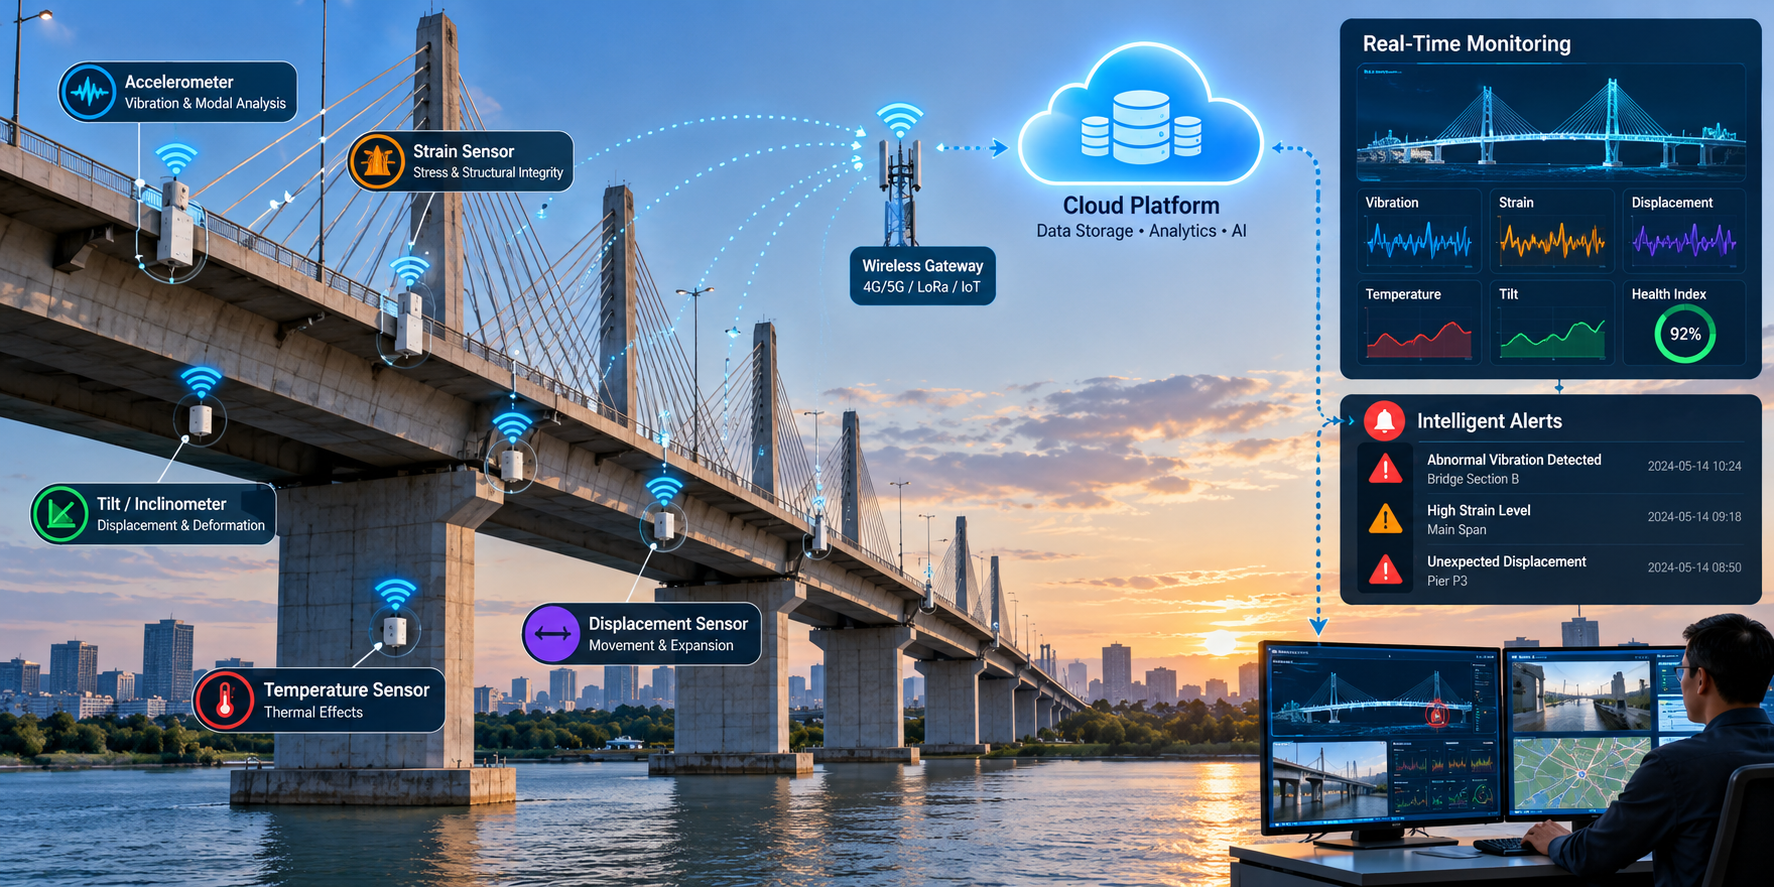
\includegraphics[width=\linewidth]{figures/ch11/ch11-02-v1-vague.png}};
\begin{scope}[x={(img.south east)},y={(img.north west)}]
  \tikzset{issuemark/.style={draw=Ch11IssueRed,line width=0.9pt,rounded corners=2pt,fill=white,fill opacity=0.90,text opacity=1,text=Ch11IssueRed,font=\sffamily\bfseries\scriptsize,inner sep=1.5pt}}
  \node[issuemark] at (0.35,0.62) {S1};
  \node[issuemark] at (0.24,0.82) {S2};
  \node[issuemark] at (0.55,0.84) {S3};
  \node[issuemark] at (0.95,0.64) {S4};
  \node[issuemark] at (0.78,0.44) {S5};
  \node[issuemark] at (0.64,0.76) {S6};
  \node[issuemark] at (0.62,0.28) {R1};
  \node[issuemark] at (0.64,0.91) {R2};
  \node[issuemark] at (0.11,0.56) {V1};
\end{scope}
\end{tikzpicture}
\caption{First draft from a one-line prompt (counter-example). Numbers match the issue list in Table~\ref{tab:ch11-01}: S1--S6 for scientific errors, R1--R2 for reading obstacles, and V1 for visual consistency. With more than three scientific errors, the first item on the revision sheet is to rewrite the input, not to patch this image. Base art and any text in it were generated by an image model and not checked.}\label{fig:ch11-02}
\end{figure}

\begin{table}[htbp]\centering\scriptsize
\setlength{\tabcolsep}{3pt}
\renewcommand{\arraystretch}{1.08}
\caption{Decomposing ``a bit messy and not professional enough'' in Figure~\ref{fig:ch11-02} into nine concrete issues across three levels.}\label{tab:ch11-01}
\begin{tabularx}{\linewidth}{@{}c>{\raggedright\arraybackslash}p{16mm}>{\raggedright\arraybackslash}p{21mm}YY@{}}
\toprule
\textbf{ID} & \textbf{Level} & \textbf{Location} & \textbf{Observed phenomenon} & \textbf{Why it is a problem} \\
\midrule
S1 & Scientific error & Bridge form & Drawn as a 6-pylon 3D perspective cable-stayed bridge rather than a twin-pylon 2D side view & Contradicts the twin-pylon study structure and 2D engineering elevation conventions \\
S2 & Scientific error & Bridge sensors & Only 5 callout boxes; pylon-top anemometer and GNSS missing; strain gauge points to upper cables instead of deck soffit; thermometer low on pier & Incomplete sensor inventory (cannot map to 12 required nodes) and placements violate engineering practice \\
S3 & Scientific error & Gateway--cloud link & Blue dashed line between wireless gateway and cloud platform has arrowheads at both ends & Misrepresents unidirectional data upload as an ambiguous bidirectional link \\
S4 & Scientific error & Top-right panel & Shows five fabricated waveform traces and a ``Health Index 92\%'' circular gauge & Methods schematic contains no empirical data, and SHM does not yield a single ``92\%'' score \\
S5 & Scientific error & Mid-right alert box & Lists three dated alarms for ``2024-05-14'' (Section B vibration, main-span high strain, Pier P3 displacement) & Fabricates monitoring dates, pier labels, and anomaly events absent from the study \\
S6 & Scientific error & Baked-in text & Titles, protocol names, and numbers are rasterized directly into the bitmap & Labels are scientific content; locking them into pixels prevents editing or translation \\
R1 & Reading obstacle & Scene \& lower right & Sunset, city skyline, river reflections, and a dual-monitor operator scene fill over half the frame & Photorealistic scenery and decorative UI panels drown out the sensing architecture \\
R2 & Reading obstacle & Cloud interior & Cloud contains only a database cylinder and generic ``Data Storage $\cdot$ Analytics $\cdot$ AI'' text & Omits the 3 explicit steps (cleaning $\rightarrow$ feature extraction $\rightarrow$ threshold/anomaly check) \\
V1 & Visual consistency & Sensors vs.\ badges & All bridge nodes are identical white boxes, while callouts use 5 colored circles & Sensor icons on the bridge lack shape and color coding, requiring text to tell types apart \\
\bottomrule
\end{tabularx}
\end{table}

This initial draft contains six Level 1 scientific errors alone (S1--S6). \textbf{Whenever a draft exhibits three or more Level 1 scientific errors, the first action on your revision sheet is never to patch the image in place---it is to return to the figure brief and regenerate from scratch.}

\section{Writing a Revision Sheet: One Change per Item}

Before generating our structural baseline image (V2), we define the components, sensor counts, and transmission links as a verifiable acceptance baseline (Table~\ref{tab:ch11-02}).

\begin{table}[htbp]\centering\scriptsize
\setlength{\tabcolsep}{3pt}
\renewcommand{\arraystretch}{1.08}
\caption{Object and relation inventory for the cable-stayed bridge SHM schematic (acceptance baseline from V2 onward).}\label{tab:ch11-02}
\begin{tabularx}{\linewidth}{@{}l>{\raggedright\arraybackslash}p{24mm}c>{\raggedright\arraybackslash}p{33mm}Y@{}}
\toprule
\textbf{ID} & \textbf{Object / relation} & \textbf{Count} & \textbf{Location (side view)} & \textbf{Visual \& line convention (text-free base)} \\
\midrule
B1--B2 & Deck girder \& pylons & 1, 2 & Left $70\%$; pylons at $x\approx 0.22, 0.50$ & Light-gray horizontal girder; medium-gray vertical single-column pylons \\
B3 & Stay cables & 16 & 4 left and 4 right per pylon, fanning from upper pylon to deck & Thin dark-gray straight lines; all connect pylon to deck, none touching water or ground \\
B4--B5 & Piers \& water band & 4, 1 & Foundations under pylons + two end piers; bottom water zone & Gray pier supports; pale-blue horizontal water band \\
S1--S5 & Accelerometers & $3+2$ & Main-span deck at $1/4, 1/2, 3/4$ (3) + midpoint of longest outer cables (2) & Small blue squares (each with a tiny black dot beside it representing wireless node N) \\
S6--S7 & Strain gauges & 2 & Underside of deck at mid-main span and next to left pylon & Small green rectangles \\
S8 / S9 & Anemometer / GNSS & 1 / 1 & Top of left pylon (S8) / top of right pylon (S9) & Small cup-anemometer icon / small dish-antenna icon \\
S10 / S11--S12 & Thermometer / displacement & $1 / 2$ & Left side-span deck (1) / both deck-end expansion joints (2) & Small round thermometer icon / small purple squares \\
G / C / P / D & Gateway / cloud / steps / terminal & 1/1/3/1 & Right $30\%$ data-path zone & Right-bank cabinet with antenna (G); cloud with server bars and 3 serial empty boxes (C, P); far-right monitor + phone (D) \\
L1 & Wireless links & Multiple & Sensor nodes N $\rightarrow$ gateway G & Short orange dashed lines with wave marks, clearly distinct from stay cables \\
L2 / L3 / L4 & Upload / steps / alert & 1 / 2 / 1 & G$\rightarrow$C / between P boxes / last P box$\rightarrow$D & Solid orange arrow / small dark-gray arrows / solid red arrow (only red element in figure) \\
\bottomrule
\end{tabularx}
\end{table}

In the \scidraw{} Scientific Figure Workflow wizard (\sdtool{figure-workflow}), we select the ``Mechanism and Workflow Diagrams'' track, populate the template with the following brief, download a copy, and generate the base image in the workflow diagram generator (\sdtool{workflow-diagram-generator}) or prompt drawing tool (\sdtool{ai-drawing}):

\begin{Prompt}
[Purpose & Audience] System schematic for Chapter 2 (Methods) of a civil engineering
master's thesis; full-page print width ~160 mm for structural engineering peers.
[Goal] Show where 12 sensors of 6 types sit on a twin-pylon cable-stayed bridge, how
wireless nodes forward data to an on-site gateway and cloud analytics pipeline, and
how threshold/anomaly alerts reach operators for engineering review.
[Basis] Farrar & Worden 2007; Ko & Ni 2005; Lynch & Loh 2006. Simplified teaching
architecture, not a real bridge, containing no empirical monitoring data.
[Objects] See inventory B1-B5, S1-S12, G, C, P, D: twin pylons, 16 stay cables (4 per
side of each pylon), 12 sensors (same type = same shape and color) with black node dots.
[Relations] L1 wireless: short orange dashed lines with wave marks (sensor -> gateway),
distinct from gray stay cables; L2 upload: solid orange arrow (gateway -> cloud);
L3 processing: 2 dark-gray arrows across 3 cloud boxes; L4 alert: solid red arrow
(last box -> terminal; red used nowhere else).
[Layout & Style] Landscape 2:1, flat 2D schematic on white, no 3D or gradients. Left
70% bridge elevation; right 30% gateway, cloud, terminal; bottom 10% empty for legend.
[Restrictions] Zero text/letters/numbers in base art; no vehicles, city, curves, cracks,
suspension main cables, cloud-to-sensor arrows, or direct sensor-to-phone arrows.
\end{Prompt}

We then convert this brief into a structured English prompt (key excerpt below; the full prompt is in the book repository's \texttt{cases/} directory):

\begin{Prompt}
Flat 2D engineering schematic, landscape 2:1, pure white background, clean vector
style, flat fills, thin dark gray outlines, no gradients, no shadows, no 3D.
ABSOLUTELY NO TEXT: no letters, words, numbers, symbols, labels, legend or title.
LEFT 70% - SIDE VIEW OF A TWIN-PYLON CABLE-STAYED BRIDGE (no main cable, no hangers):
- Pale blue water band (y 0.75-0.88); light gray deck girder (x 0.03-0.68, y 0.60-0.63);
  two medium gray vertical pylons at x 0.22 and x 0.50 on gray piers; two end piers.
- Exactly 16 straight thin dark gray stay cables: 4 left and 4 right on each pylon,
  every cable connecting pylon to deck, none touching water or ground.
- SENSORS (12 total, each with a tiny black wireless node dot beside it):
  3 blue squares on main-span deck (1/4, 1/2, 3/4); 2 blue squares on longest outer
  cables; 2 green rectangles under deck; 1 cup anemometer on left pylon top; 1 dish
  GNSS antenna on right pylon top; 1 round thermometer on left side span; 2 purple
  squares at both deck ends.
RIGHT 30% - DATA PATH: gateway cabinet with antenna on right bank; cloud outline with
3 server bars and 3 empty rounded processing boxes connected by dark gray arrows;
operator terminal (monitor + phone) at far right.
LINES: short orange dashed wireless lines with wave marks from sensors to gateway;
one solid orange upload arrow (gateway -> cloud); one solid red alert arrow (last box
-> terminal; red used nowhere else). Keep bottom 10% empty for legend.
\end{Prompt}

We ran this exact prompt three times and audited each output at $200\%$ zoom against Table~\ref{tab:ch11-02}. In the first run, only $3+3+3+3=12$ stay cables connected to the pylon shafts, while the outer-left blue cable accelerometer sat on a detached diagonal segment whose upper end floated in mid-air; we rejected it. In the third run, all 16 cable trajectories and 12 sensors appeared, but main-span cables crossed in a crowded tangle, the left-pylon cup anemometer was painted blue like the accelerometers, the gateway cabinet floated without bank support, and the cloud pressed into the water band; we rejected it as well. The second run (Figure~\ref{fig:ch11-03}) preserved the twin-pylon side view, 16 stay-cable trajectories connecting pylons to the deck, all 12 sensors with adjacent black node dots, the gateway, cloud, three processing boxes, terminal, and all four arrow directions, with zero text. We selected this second run as our \textbf{candidate structural baseline (V2)} for subsequent comparisons.

\begin{figure}[htbp]\centering
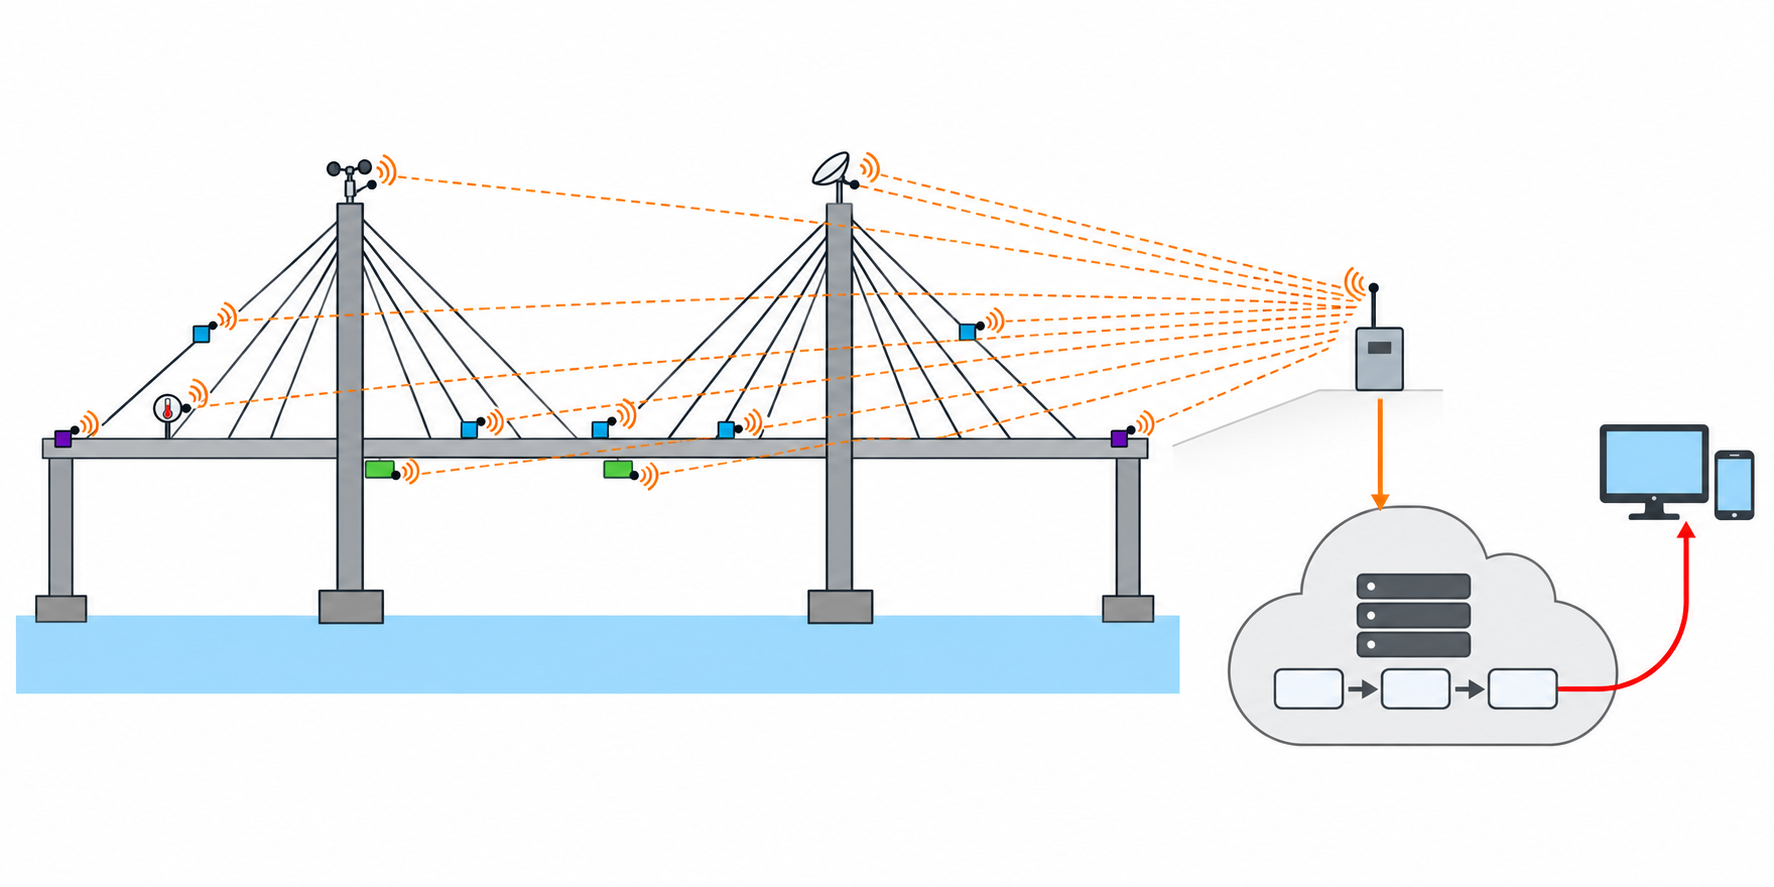
\includegraphics[width=\linewidth]{figures/ch11/ch11-03-v2-brief.png}
\caption{Candidate structural baseline V2 generated from the full brief (second generation run). The twin-pylon bridge form, 16 stay-cable trajectories, 12 sensors, right-hand subsystems, and semantic arrow directions match Table~\ref{tab:ch11-02} with zero baked-in text, serving as the reference baseline for all later versions. However, several reading and consistency flaws remain: the orange wireless dashes are thin, the cloud sits below the gateway, the thermometer icon contains red fill, sensor icons are slightly undersized, and narrow white gaps appear where stay cables pass behind icons (see Table~\ref{tab:ch11-03}). Base art generated by an image model.}\label{fig:ch11-03}
\end{figure}

V2 is a comparison baseline rather than an accepted final figure. Auditing Figure~\ref{fig:ch11-03} against our brief yields the structured \textbf{revision sheet} in Table~\ref{tab:ch11-03}, where every item records its ID, level, location, observed phenomenon, revision requirement, \textbf{what must remain unchanged}, and execution channel.

\begin{table}[htbp]\centering\scriptsize
\setlength{\tabcolsep}{3pt}
\renewcommand{\arraystretch}{1.08}
\caption{Revision sheet compiled from the audit of candidate baseline V2 (Figure~\ref{fig:ch11-03}).}\label{tab:ch11-03}
\begin{tabularx}{\linewidth}{@{}c>{\raggedright\arraybackslash}p{14mm}>{\raggedright\arraybackslash}p{18mm}YYY>{\raggedright\arraybackslash}p{18mm}@{}}
\toprule
\textbf{ID} & \textbf{Level} & \textbf{Location} & \textbf{Observed phenomenon \& impact} & \textbf{Revision requirement} & \textbf{Must remain unchanged} & \textbf{Channel} \\
\midrule
R2 & Reading obstacle & Sensor-to-gateway lines & Orange wireless dashes are thin and lose contrast across stay-cable fans & Change to thicker orange short-dashed lines with wave marks, distinct from dark-gray stay cables & Bridge form, 16 stay cables, 12 sensors, gateway, cloud, terminal, and L2--L4 & Image model (reference edit); TikZ if 2 runs fail \\
R3 & Reading obstacle & All 12 sensors & Blue squares measure $\sim 1.44\text{--}1.80\ \text{mm}$ at $160\ \text{mm}$ width ($<2\ \text{mm}$) & Enlarge sensor icons by $\sim 1.5\times$ (executed separately from R2) & All bridge components, cables, and links as above & Image model (separate round) or vector overlay \\
R4 & Reading obstacle & Right data path & Gateway sits high ($y\approx 0.41$) and cloud sits low ($y\approx 0.71$); upload arrow points down & Adapt label coordinates to actual layout for demo; swap gateway/cloud vertically before submission & Left $70\%$ bridge, 16 stay cables, and 12 sensors & Layout layer adaptation or right-zone redraw \\
V1 & Visual consistency & Thermometer \& blue squares & Thermometer has red fill (violating single-use alert red); blue hex values unverified & Recolor thermometer interior to gray; unify accelerometer blues (e.g., \texttt{\#4C78A8}) & Other sensor icons, structural grays, and red alert arrow & Post-process in vector / image editor \\
V2 & Visual consistency & Cable crossings \& water & Narrow white halo gaps interrupt cables behind icons/waves; mild gradients on water/screen & Bridge cable gaps and flatten gradients in vector or raster editor before submission & Endpoints of all 16 stay cables and sensor positions & Layout layer / vector editor \\
T1 & Labels \& legend & Full canvas \& bottom & Base art has no text; needs component names, subsystem labels, and legend & Overlay 7 labels and a bottom legend in LaTeX/TikZ at measured coordinates & Base bitmap pixels untouched & Layout layer (TikZ) \\
\bottomrule
\end{tabularx}
\end{table}

\begin{BookNote}
\textbf{Three rules for writing a revision sheet:} (1) \textbf{Change only one class of issue at a time}---never bundle thicker dashed lines, larger sensor icons, and a gateway--cloud position swap into a single prompt; (2) \textbf{State an explicit ``must remain unchanged'' inventory}, replacing vague phrases like ``keep everything else the same'' with exact object names and counts; and (3) \textbf{Handle typography, exact color values, gap repairs, and alignment in the layout layer} rather than gambling on repeated generative redraws.
\end{BookNote}

\section{Collateral Changes from Local Edits: How to Spot Them}

Why does Table~\ref{tab:ch11-03} restrict generative edits so tightly? Because a ``local edit'' in a generative image model is not a localized operation on an isolated vector path. When you select a prior image in \scidraw{} (\sdtool{ai-drawing}) as a reference image and submit a modification prompt, the model conditions on both the reference bitmap and your text instruction to \textbf{resynthesize the entire canvas}. There is no ``object locking'' or ``regional pixel freeze'' in generative image editing; as the model redraws the targeted feature, it can silently alter, shift, or drop unmentioned objects---causing \textbf{collateral changes}.

\subsection{Real Case 1: A Style Revision in Chapter 7 Altered Five Structural Features}

Consider first the real iteration record from Chapter 7's mechanism schematic of insulin-stimulated GLUT4 translocation (Figure~\ref{fig:ch11-07}). Its V2 baseline (Figure~\ref{fig:ch11-07}, left) had already verified all 13 signaling objects, 6 amber phosphorylation dots, and five arrow styles. For V3, the author requested only Level 3 stylistic cleanup---unifying protein blue hues, standardizing line weights, and adding whitespace---while specifying ``keep the exact same content and layout.''

When the first V3 run was submitted without attaching the V2 bitmap as a reference image (Figure~\ref{fig:ch11-07}, middle), the colors and strokes became cleaner, but five severe structural collateral changes appeared simultaneously: (a) all six phosphorylation dots on the receptor, IRS-1, Akt, and AS160 vanished; (b) insulin dropped from three beads to two and detached from the receptor; (c) PDK1 and Akt detached from the inner leaflet of the plasma membrane into the cytosol; (d) an unrequested solid activation arrow appeared between PI3K and PDK1; and (e) each storage vesicle acquired multiple GLUT4 barrels instead of one, alongside stray intracellular glucose hexagons. Only in the second run, when V2 was passed as a reference image (Figure~\ref{fig:ch11-07}, right), were the main structure and phosphorylation dots preserved. Even with a reference image attached, Chapter 7's palette counter-example experiment showed the model quietly turning the open arrowhead on the $\text{PIP}_2 \rightarrow \text{PIP}_3$ conversion arc into a filled arrowhead.

\begin{figure}[htbp]\centering
% FIG ch11-07 Chapter 7 collateral reuse (English)
\usetikzlibrary{arrows.meta,calc}
\begin{tikzpicture}
  \def\panelW{0.31\linewidth}
  \definecolor{Ch11AnnotRed}{HTML}{C0392B}
  \node[anchor=south west, inner sep=0] (imA) at (0,0) {%
    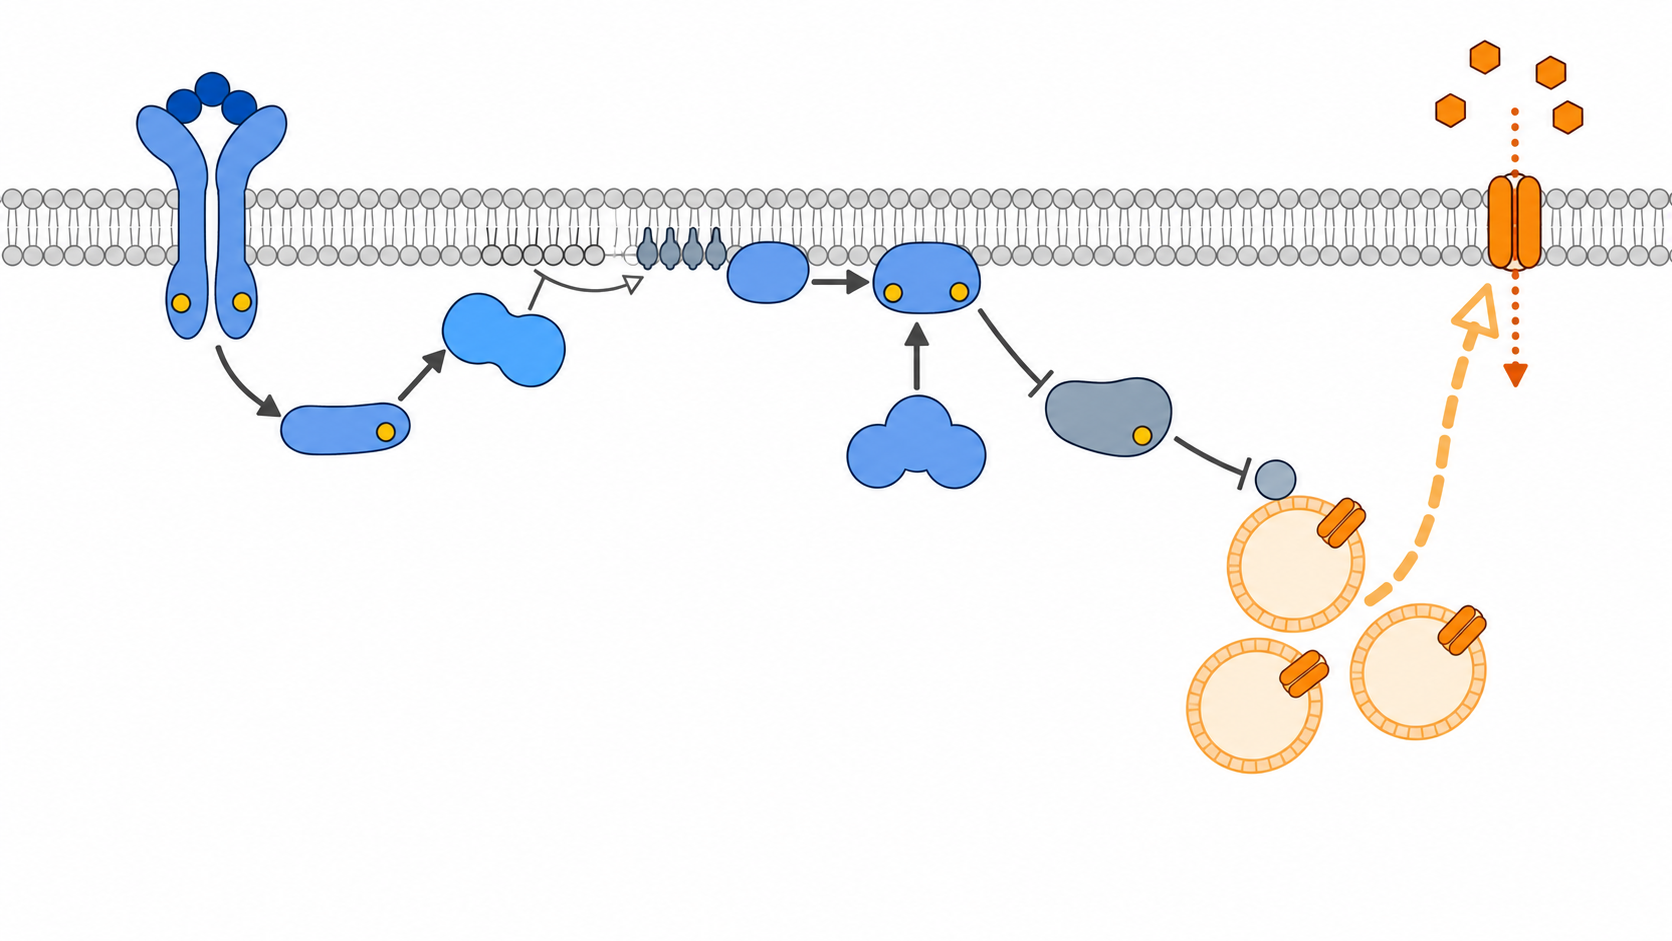
\includegraphics[width=\panelW]{figures/ch11/ch11-07a-ch07-v2.png}};
  \node[font=\small\sffamily, anchor=south] at ($(imA.north)+(0,2mm)$) {V2 baseline};

  \node[anchor=south west, inner sep=0] (imB) at (0.345\linewidth,0) {%
    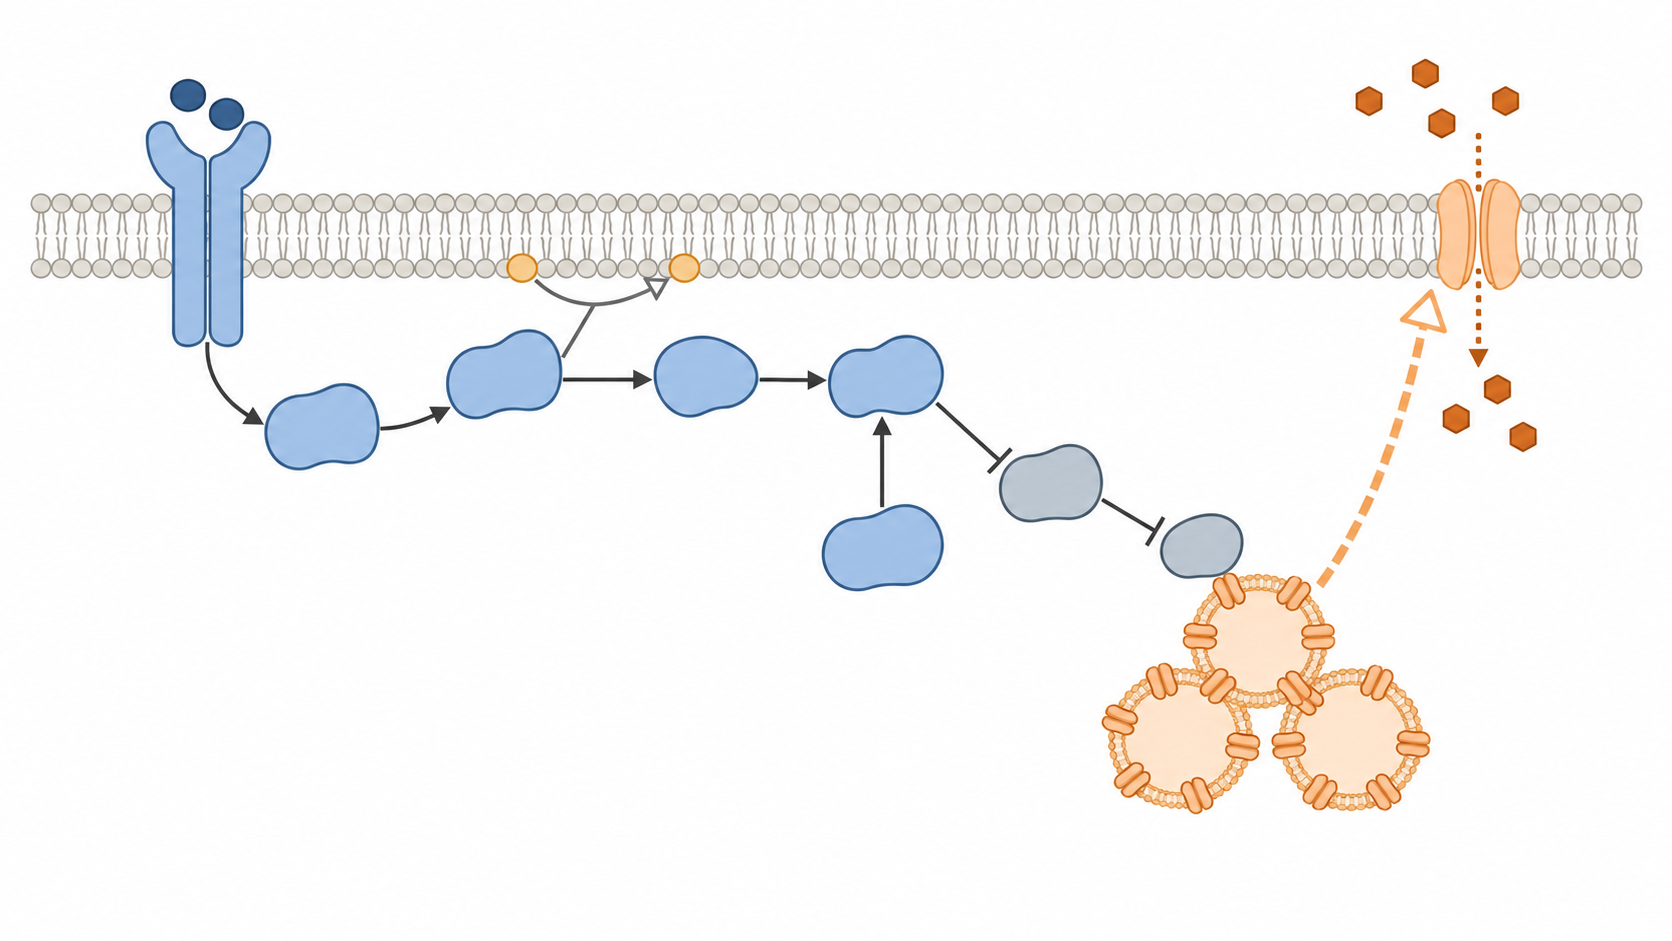
\includegraphics[width=\panelW]{figures/ch11/ch11-07b-ch07-v3-alt1.png}};
  \node[font=\small\sffamily, anchor=south] at ($(imB.north)+(0,2mm)$) {V3, attempt 1 (rejected)};
  \begin{scope}[x={(imB.south east)},y={(imB.north west)}]
    \draw[Ch11AnnotRed, line width=0.7pt] (0.11,0.28) circle (0.035);
    \node[font=\scriptsize\sffamily, text=Ch11AnnotRed, anchor=west] at (0.15,0.28) {(a)};
    \draw[Ch11AnnotRed, line width=0.7pt] (0.10,0.08) circle (0.04);
    \node[font=\scriptsize\sffamily, text=Ch11AnnotRed, anchor=west] at (0.14,0.08) {(b)};
    \draw[Ch11AnnotRed, line width=0.7pt] (0.48,0.38) circle (0.06);
    \node[font=\scriptsize\sffamily, text=Ch11AnnotRed, anchor=west] at (0.54,0.38) {(c)};
    \draw[Ch11AnnotRed, line width=0.7pt] (0.34,0.36) circle (0.045);
    \node[font=\scriptsize\sffamily, text=Ch11AnnotRed, anchor=west] at (0.39,0.36) {(d)};
    \draw[Ch11AnnotRed, line width=0.7pt] (0.76,0.70) circle (0.07);
    \node[font=\scriptsize\sffamily, text=Ch11AnnotRed, anchor=west] at (0.82,0.70) {(e)};
  \end{scope}

  \node[anchor=south west, inner sep=0] (imC) at (0.69\linewidth,0) {%
    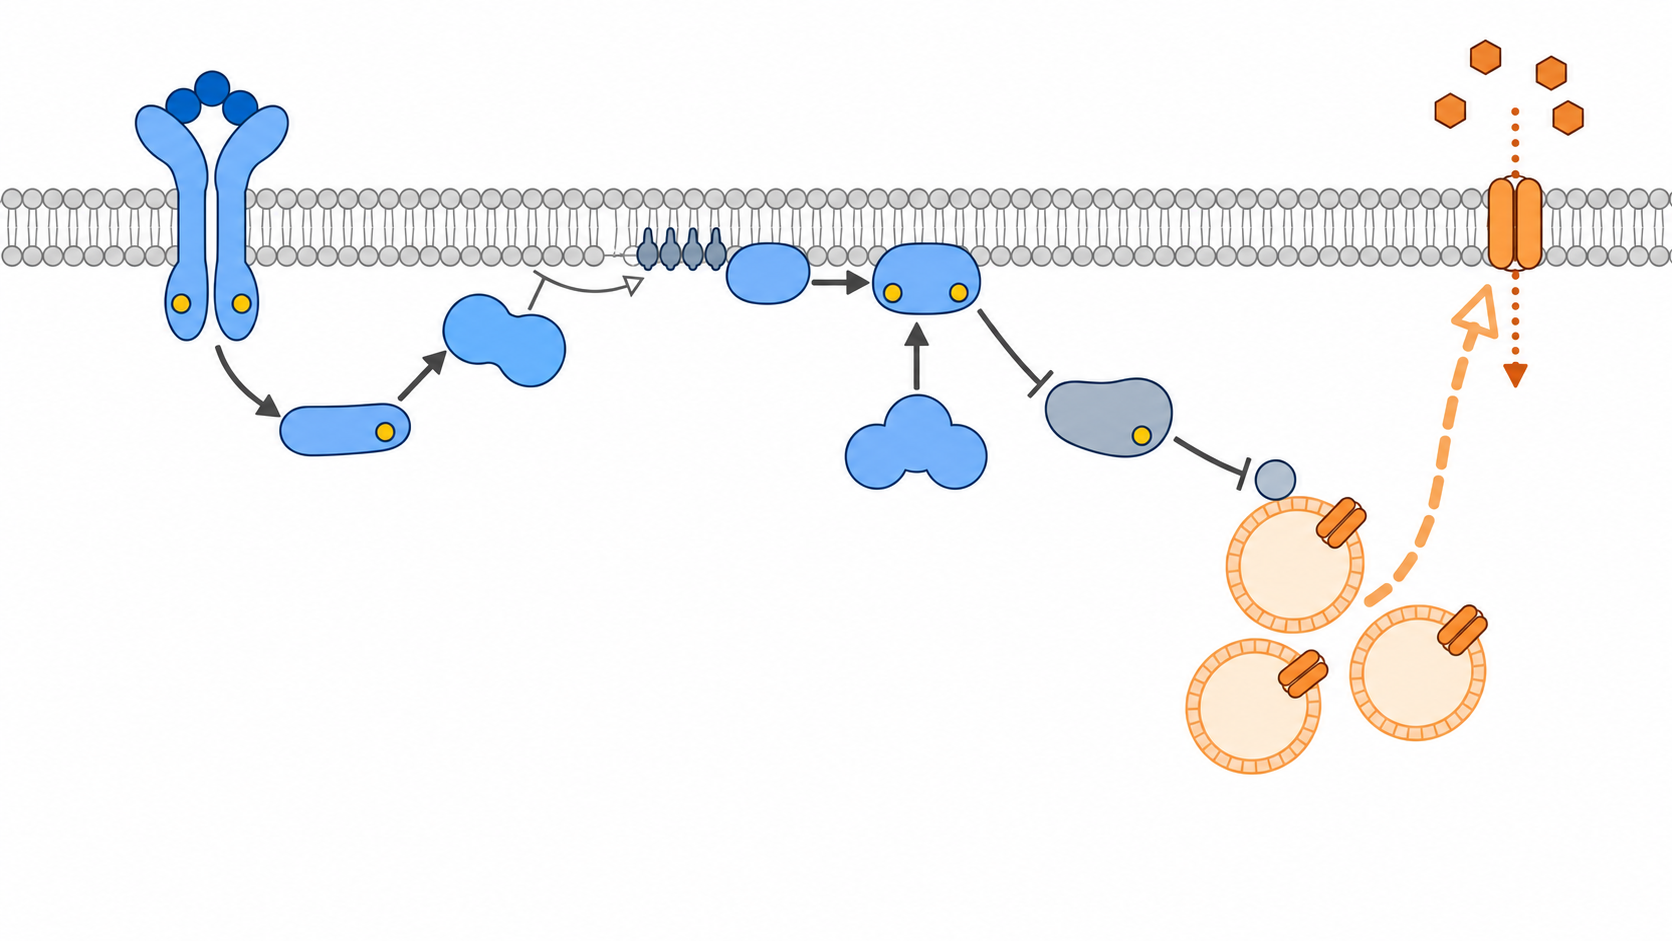
\includegraphics[width=\panelW]{figures/ch11/ch11-07c-ch07-v3.png}};
  \node[font=\small\sffamily, anchor=south] at ($(imC.north)+(0,2mm)$) {V3, attempt 2 (accepted)};
\end{tikzpicture}

\caption{A real iteration from Chapter 7: an instruction about colour and line style can still change the structure. Left, V2 baseline. Middle, V3 attempt 1 (generated from the revised prompt without a reference image): (a) all phosphorylation marks lost; (b) insulin reduced from three beads to two and detached from the receptor; (c) PDK1 and Akt moved off the membrane; (d) an unrequested PI3K$\rightarrow$PDK1 activation arrow added; (e) several GLUT4 per vesicle instead of one. Right, attempt 2 of the same instruction with V2 passed as a reference image keeps the main structure but still needs a full check. All three generated by an image model.}\label{fig:ch11-07}
\end{figure}

\subsection{Real Case 2: Three Reference-Image Revision Runs for V3 in This Chapter}

Now examine item R2 on our revision sheet. Inside \scidraw{} (\sdtool{ai-drawing}), we select V2 (Figure~\ref{fig:ch11-03}) from the history as our reference image and formulate a single-issue instruction targeting only the wireless links:

\begin{Prompt}
Target edit (Item R2): Change only the wireless transmission lines from the sensors
to the gateway into thicker orange short-dashed lines with small wave marks so they
are immediately distinguishable from the stay cables. Keep everything else unchanged.
\end{Prompt}

The exact English prompt submitted with V2 attached as the reference image was:

\begin{Prompt}
Using the reference image, change only the wireless lines from the sensors to
the gateway: make them thicker orange short-dashed lines with small wave marks,
so they cannot be confused with the stay cables. Keep everything else
unchanged. No text.
\end{Prompt}

We executed three independent reference-image edits from V2, auditing all objects against Table~\ref{tab:ch11-02} each time. Figure~\ref{fig:ch11-04} compares V2 (left) with V3 attempt 1 (right).

\begin{figure}[htbp]\centering
\resizebox{\linewidth}{!}{%
\begin{tikzpicture}
\definecolor{Ch11OkGreen}{HTML}{2E8B57}
\definecolor{Ch11WarnRed}{HTML}{C0392B}
\node[anchor=south west,inner sep=0] (imL) at (0,0) {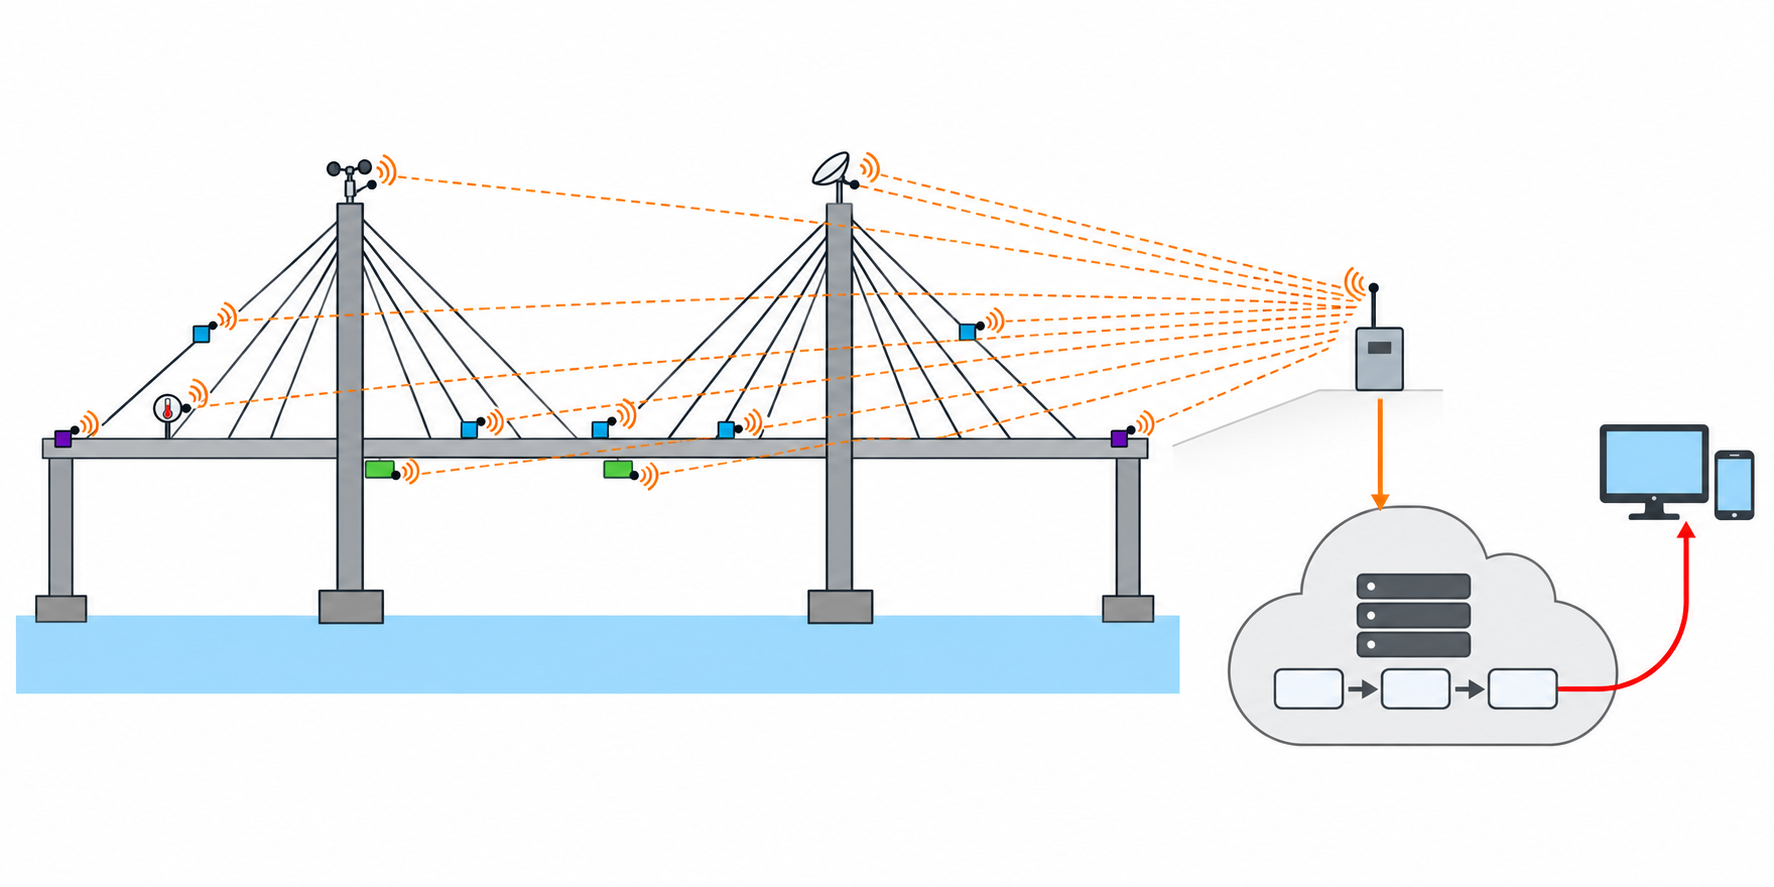
\includegraphics[width=0.488\linewidth]{figures/ch11/ch11-03-v2-brief.png}};
\node[font=\sffamily\footnotesize,anchor=south] at ($(imL.north)+(0,1.5mm)$) {V2 candidate baseline (before edit)};
\node[anchor=south west,inner sep=0] (imR) at (0.512\linewidth,0) {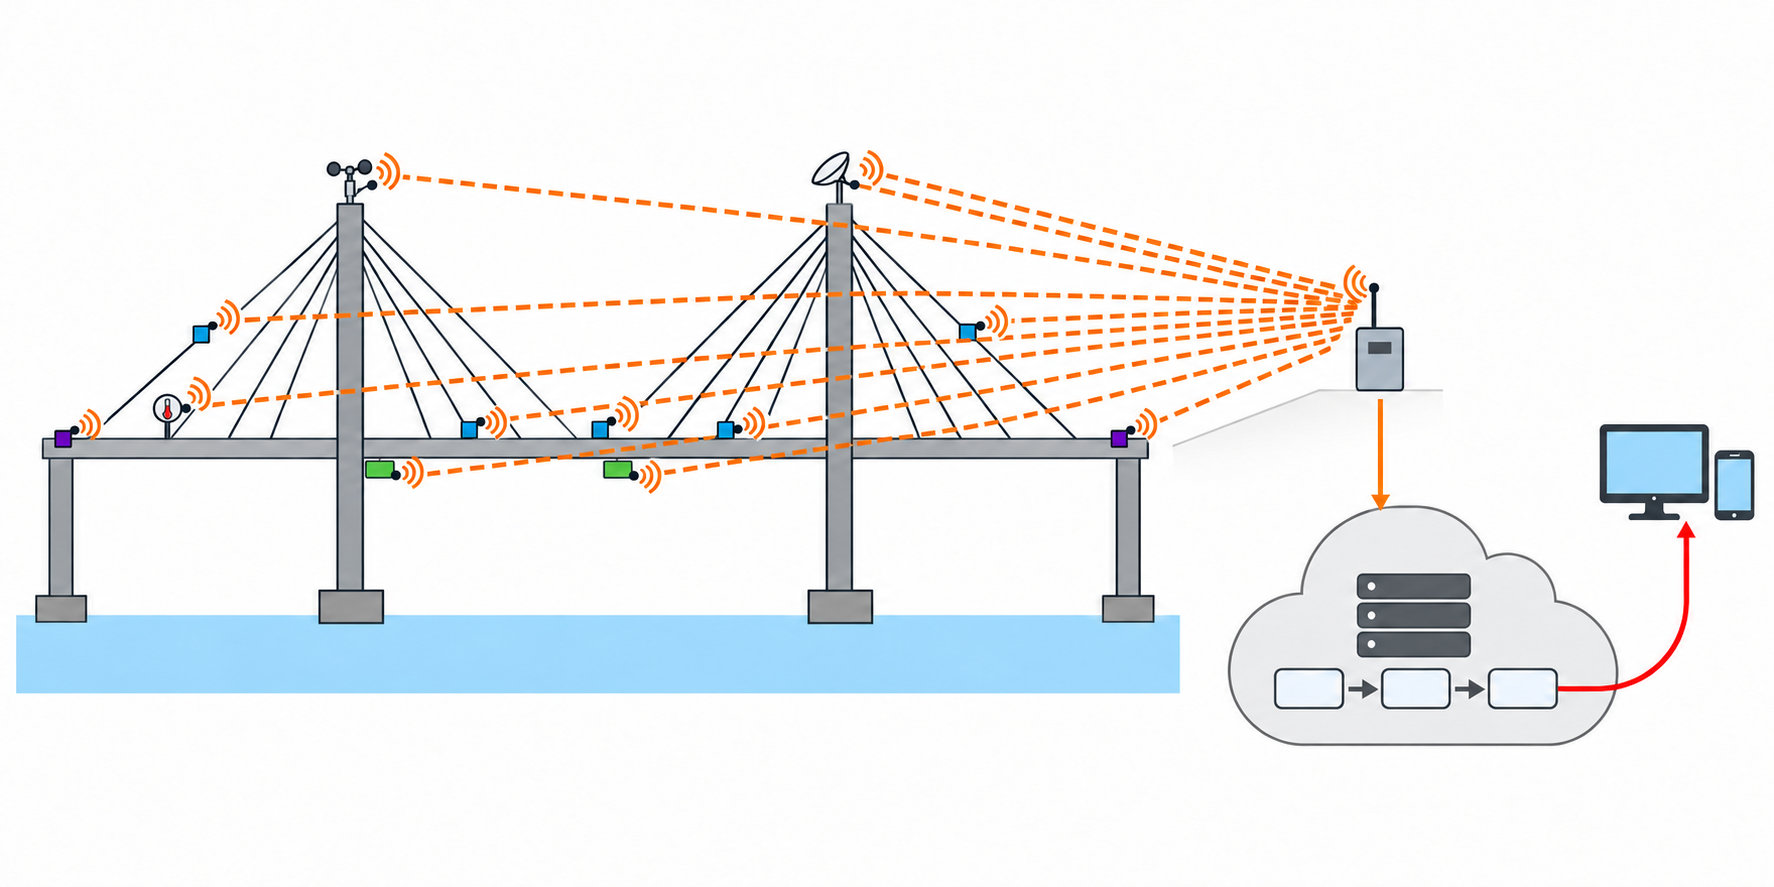
\includegraphics[width=0.488\linewidth]{figures/ch11/ch11-04-v3-collateral.png}};
\node[font=\sffamily\footnotesize,anchor=south] at ($(imR.north)+(0,1.5mm)$) {V3, attempt 1 (after reference-image edit)};
\begin{scope}[x={(imR.south east)},y={(imR.north west)}]
  \draw[Ch11OkGreen,line width=0.9pt,rounded corners=2pt] (0.50,0.61) rectangle (0.76,0.80);
  \node[fill=white,fill opacity=0.9,text opacity=1,text=Ch11OkGreen,font=\sffamily\bfseries\scriptsize,inner sep=1pt,anchor=south] at (0.63,0.81) {Target edit done: thicker orange dashes};
  \draw[Ch11WarnRed,dashed,line width=0.7pt,rounded corners=2pt] (0.06,0.49) rectangle (0.13,0.59);
  \node[fill=white,fill opacity=0.9,text opacity=1,text=Ch11WarnRed,font=\sffamily\scriptsize,inner sep=1pt,anchor=south] at (0.10,0.60) {Inherited flaw 1};
  \draw[Ch11WarnRed,dashed,line width=0.7pt,rounded corners=2pt] (0.68,0.14) rectangle (0.91,0.44);
  \node[fill=white,fill opacity=0.9,text opacity=1,text=Ch11WarnRed,font=\sffamily\scriptsize,inner sep=1pt,anchor=north] at (0.80,0.13) {Inherited flaw 2: cloud below gateway};
\end{scope}
\end{tikzpicture}}
\caption{V3 attempt 1 (right), produced by asking only for a change to the wireless lines, beside the candidate baseline V2 (left). The solid green box marks the completed target edit (thicker orange short-dashed lines and clearer wave marks near sensor nodes). Across three independent reference-image edits, all 16 stay-cable trajectories and 12 sensors were preserved without observable structural collateral changes, though a full-figure check was required to confirm this. Dashed red boxes mark pre-existing baseline flaws inherited unchanged from V2 (red fill inside the thermometer and the cloud positioned below the gateway). Base art generated by an image model without manual alteration.}\label{fig:ch11-04}
\end{figure}

The three empirical runs establish three points: (1) \textbf{Target edit completed:} all three runs thickened the orange short-dashed lines and made the wave marks near the sensor nodes more prominent, clearly distinguishing radio links from the thin dark-gray stay cables (though waves stayed near the nodes rather than along mid-span segments); (2) \textbf{No structural collateral changes observed across all three runs:} 2 pylons, 16 stay-cable trajectories ($4+4+4+4$), 12 sensors ($3+2+2+1+1+1+2$), the gateway, cloud, 3 processing boxes, terminal, and arrows L2--L4 remained consistent with V2; and (3) \textbf{Pre-existing V2 flaws were inherited unchanged:} the red thermometer interior (Inherited flaw 1), the cloud below the gateway (Inherited flaw 2), small sensor icons, and narrow white cable gaps persisted in all three outputs.

This demonstrates the stochastic nature of generative edits: \textbf{``no collateral change occurred this time'' is a conclusion you can state only after a full item-by-item count, never an assumption you can make beforehand.}

\subsection{Verifying with Side-by-Side Comparison, Pixel Difference Maps, and Object Count Tables}

Catching collateral changes relies on combining three complementary methods (Figure~\ref{fig:ch11-05}):

\begin{figure}[htbp]\centering
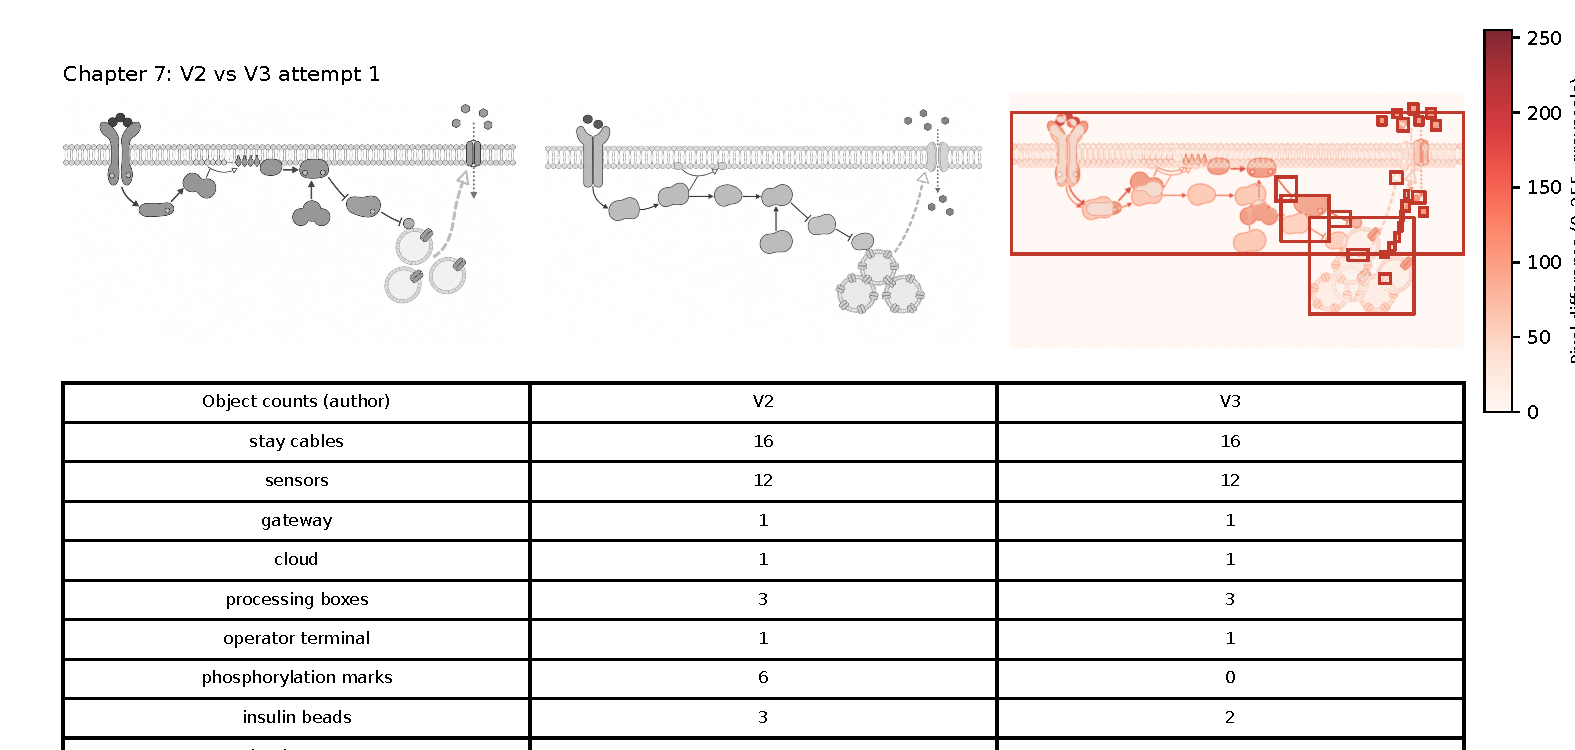
\includegraphics[width=\linewidth]{figures/ch11/ch11-05-diff-and-count-en.pdf}
\caption{Finding collateral changes with a difference map and an object count. The difference map shows where grayscale pixels changed between two versions. When the layout is preserved it points straight at altered or missing objects; when the whole image is redrawn and repositioned (top row: Chapter 7's V2 and the first V3 attempt), difference bounding boxes cover everything (24 regions across $14.6\%$ of pixels) and only an object-by-object count still works (bottom table: first 6 rows for this chapter's V2 vs.\ V3; last 4 rows for Chapter 7). Counts were made by the author.}\label{fig:ch11-05}
\end{figure}

First, \textbf{same-scale side-by-side comparison or rapid blink toggling}. Because \scidraw{} does not currently include an in-app side-by-side comparator, download the old and new versions and align them at equal width (as in Figure~\ref{fig:ch11-04}), or flip rapidly between them in an image viewer so any displaced or missing element flickers into view.

Second, \textbf{pixel difference heatmaps and their limitation}. After scaling two versions to equal dimensions and converting them to grayscale ($0\text{--}255$), you compute the absolute pixel difference, apply a Gaussian blur (radius $\approx 2\ \text{px}$) to suppress anti-aliasing noise, and box connected regions exceeding a difference of $40$. When background coordinates stay fixed, the heatmap pinpoints altered lines; when the model rearranges the layout globally---as in Chapter 7's V2 versus V3 attempt 1 (top row of Figure~\ref{fig:ch11-05})---$14.6\%$ of pixels exceed the threshold and 24 red boxes blanket the canvas, losing localization power.

Third, \textbf{the manual object count table (the final line of defense)}. Counting entities row by row against the inventory table (bottom of Figure~\ref{fig:ch11-05}) confirms that our bridge V2 and V3 match across stay cables ($16/16$), sensors ($12/12$), gateway ($1/1$), cloud ($1/1$), processing boxes ($3/3$), and terminal ($1/1$). In contrast, Chapter 7's V2 versus V3 attempt 1 drops phosphorylation dots from $6$ to $0$ and insulin beads from $3$ to $2$, while increasing activation arrows from $4$ to $5$ and maximum GLUT4 per vesicle from $1$ to $3$. Difference maps assist the eye, but manual table counts safeguard the science.

\section{Branching Back to the Previous Version, and When to Move to the Layout Layer}

Once an audit uncovers a collateral change (such as a missing antenna or lost stay cable), never stay on the broken V3 and prompt ``add the missing antenna back.'' As the dashed box at the lower right of Figure~\ref{fig:ch11-08} illustrates, stacking patches onto a defective version ($\text{V3} \rightarrow \text{V3}' \rightarrow \text{V3}''$) causes each full-canvas redraw to introduce fresh drift, compounding errors until their origin is untraceable.

\begin{figure}[htbp]\centering
\resizebox{\linewidth}{!}{\tikzset{every node/.append style={align=center}}% FIG ch11-08 version tree (English)
\usetikzlibrary{arrows.meta,positioning,fit,calc}
\definecolor{Ch11BadRed}{HTML}{C0392B}
\definecolor{Ch11GoodGreen}{HTML}{2E8B57}
\providecommand{\ChElevenThumb}[2]{%
  \IfFileExists{#1}{%
    \includegraphics[width=24mm]{#1}%
  }{%
    \fbox{\parbox[c][16mm][c]{24mm}{\centering\scriptsize\sffamily #2\\{\tiny (base pending)}}}}%
}
\begin{tikzpicture}[
  x=1mm, y=1mm,
  font=\sffamily\footnotesize,
  edge/.style={draw=BookInk!60, -{Stealth[length=2mm]}, line width=0.55pt},
  badedge/.style={draw=Ch11BadRed!70, dashed, -{Stealth[length=2mm]}},
  nlabel/.style={align=center, text width=26mm, font=\scriptsize},
]
  \node (V1) at (0,0) {\ChElevenThumb{figures/ch11/ch11-02-v1-vague.png}{V1}};
  \node[nlabel, below=1mm of V1] {One-line prompt};

  \node (V2) [below=14mm of V1] {\ChElevenThumb{figures/ch11/ch11-03-v2-brief.png}{V2\\baseline}};
  \node[nlabel, below=1mm of V2] {\textbf{Structural baseline}};

  \node (V3) [below=14mm of V2] {\ChElevenThumb{figures/ch11/ch11-04-v3-collateral.png}{V3}};
  \node[nlabel, below=1mm of V3, text=Ch11BadRed] {Collateral change\\{\tiny (rejected)}};

  \node (V4) at (42,-28) {\ChElevenThumb{figures/ch11/ch11-06-v4-recovered.png}{V4}};
  \node[nlabel, below=1mm of V4, text=Ch11GoodGreen] {Back to V2\\wireless lines only};

  \node (Final) at (84,-28) {\ChElevenThumb{figures/ch11/ch11-06-v4-recovered.png}{Final}};
  \node[nlabel, below=1mm of Final] {TikZ labels \& legend};

  \draw[edge] (V1) -- node[left, font=\tiny, align=right] {Rewrite\\input} (V2);
  \draw[edge] (V2) -- node[right=1.5mm, font=\tiny, align=left] {Wireless\\lines only} (V3);
  \draw[edge] (V2.east) -- node[above, font=\tiny] {Wireless +\\keep list} (V4.west);
  \draw[edge] (V4.east) -- node[above, font=\tiny] {Labels \&\\legend} (Final.west);

  \node[draw=Ch11BadRed, dashed, rounded corners=2pt, inner sep=4pt, fit=(V3)] {};
  \node[font=\scriptsize, text=Ch11BadRed, right=1mm of V3] {×};

  \node (Vp1) at (42,-66) {\fbox{\parbox[c][16mm][c]{24mm}{\centering\scriptsize V3$'$\\schematic}}};
  \node[font=\tiny, below=1mm of Vp1, text width=28mm, align=center] {Add back missing antenna};
  \node (Vp2) [right=12mm of Vp1] {\fbox{\parbox[c][16mm][c]{24mm}{\centering\scriptsize V3$''$\\schematic}}};
  \node[font=\tiny, below=1mm of Vp2, text width=28mm, align=center] {Another drift};
  \draw[badedge] (Vp1) -- (Vp2);
  \node[draw=BookInk!40, dashed, rounded corners=2pt, inner sep=6pt,
    fit=(Vp1)(Vp2), label={[font=\scriptsize, yshift=2mm]above:Wrong: patch the faulty version}] {};
  \draw[badedge] (V3.east) -- ++(6,0) |- (Vp1.west);
\end{tikzpicture}
}
\caption{Version tree for this chapter's case. When a revision shows collateral changes, do not patch the faulty version; return to the V2 baseline and branch again (V4), restating what must stay and changing one thing. The dashed box shows how patching a faulty version piles up problems that are hard to trace. (Note: our three V3 runs did not lose structural objects; the V3 branch here illustrates the standard rollback logic when collateral changes occur.)}\label{fig:ch11-08}
\end{figure}

Instead, \textbf{re-select the baseline V2 from your \scidraw{} history} to start a clean branch (V4), pairing your single modification request with an item-by-item preservation checklist:

\begin{Prompt}
Use this reference image as the basis for the edit. Change only one thing:
make the wireless transmission lines from the sensors to the gateway thicker
orange short-dashed lines with small wave marks.
The following must remain unchanged, item by item:
- The side view of the twin-pylon cable-stayed bridge; the positions, heights
  and shapes of both pylons.
- All 16 stay cables: 4 on the left and 4 on the right of each pylon, all
  connecting a pylon to the deck; their positions and angles.
- The positions, shapes and colors of all 12 sensors: 3 blue squares on the
  main-span deck; 1 blue square at the middle of each of the two longest
  outer cables; 2 green rectangles under the deck; the anemometer on top of
  the left pylon; the GNSS antenna on top of the right pylon; the thermometer
  on the left side span; and 2 purple squares at the deck ends.
- The positions of the gateway, cloud, 3 processing boxes inside the cloud,
  and operator terminal; the orange upload arrow and the red alert arrow.
- Do not add any new objects, new lines or text.
If you cannot make the edit without changing anything else, leave the
original image unchanged.
\end{Prompt}

Executing this prompt with V2 as the reference image produced the V4 base image: the orange short-dashed wireless links were thickened, all 16 stay-cable trajectories and 12 sensors were preserved, and grayscale conversion confirmed clear separation between the thick dashed wireless links and thin solid stay cables.

If a local modification still causes collateral changes twice in a row despite an explicit preservation checklist, \textbf{switch to the layout-layer route}: replace the wireless-line clause in the V2 prompt with \texttt{Do not draw any lines from sensors to the gateway}, generate a link-free base image, verify all 16 stay cables and 12 sensors, and draw the orange dashed links and wave marks in TikZ (the cost is re-auditing the new base image once; the benefit is that future line-style edits never touch the bitmap).

By contrast, data charts in \scidraw{} Scientific Visualization (\sdtool{sci-vis}) are redrawn from code or chart configurations and support conversational edits plus one-click restoration to the previous or original version without randomly dropping data points. Nevertheless, data plots still require full-figure re-verification after every edit or rollback to ensure that updated axis limits did not clip extreme values or distort statistical comparisons.

\section{Revision Logs, Overlaid Final Figure, and Full-Figure Re-Verification}

Every iteration should leave a row in your revision log recording the parent version, prompt summary, target edit, observed deviations or collateral changes, and adoption decision (Table~\ref{tab:ch11-04}).

\begin{table}[htbp]\centering\scriptsize
\setlength{\tabcolsep}{3pt}
\renewcommand{\arraystretch}{1.08}
\caption{Version-by-version revision log for the cable-stayed bridge SHM schematic case study.}\label{tab:ch11-04}
\begin{tabularx}{\linewidth}{@{}l>{\raggedright\arraybackslash}p{13mm}>{\raggedright\arraybackslash}p{21mm}YY>{\raggedright\arraybackslash}p{18mm}@{}}
\toprule
\textbf{Version} & \textbf{Based on} & \textbf{Prompt summary} & \textbf{Target change \& positive results} & \textbf{Observed deviations or collateral changes} & \textbf{Decision} \\
\midrule
V1 (1 run) & --- & One-line vague English prompt & Produced photorealistic counter-example & 6 scientific errors S1--S6 (6-pylon 3D bridge, missing anemometer/GNSS, bidirectional arrow, fabricated waveforms, ``92\%'' score, dated alarms) & Rejected; rewrite input \\
V2, run 1 & Brief & Full structured English prompt & Twin-pylon side view, 12 sensors, zero text & $200\%$ check showed only 12 stay cables reaching pylons ($3+3+3+3$) plus 1 floating diagonal segment on left & Rejected (archived alt1) \\
V2, run 2 & Brief & Same full prompt, 2nd run & 16 stay-cable trajectories, 12 sensors, subsystems, and 4 arrow directions correct; zero text & Wireless dashes thin; cloud below gateway; red inside thermometer; small sensor icons; narrow white gaps where cables cross icons & Selected as baseline V2 \\
V2, run 3 & Brief & Same full prompt, 3rd run & 16 stay-cable trajectories and 12 sensors countable & Main-span cables cross in a crowded tangle; anemometer colored blue; gateway floats; cloud presses into water band & Rejected (archived alt2) \\
V3 (3 runs) & V2 & Reference edit: thicken wireless dashes + waves & All 3 runs thickened orange short dashes and enhanced node wave marks & No missing cables or sensors across 3 runs; inherited V2's low cloud, red thermometer, small icons, and cable gaps & Run 1 shown in Fig.~\ref{fig:ch11-04} \\
V4 (1 run) & V2 & Back to V2 + wireless edit + keep list & Orange wireless dashes thickened; 16 cables and 12 sensors preserved; distinct in grayscale & No new collateral changes; still inherits V2's cloud below gateway, red thermometer, small icons, and narrow cable gaps & Selected as base for overlay \\
Overlaid final & V4 & TikZ callout labels and bottom legend & 7 structural/subsystem labels and two-row legend added at $\ge 6\ \text{pt}$ vector text & Base bitmap unretouched; 4 inherited base deviations documented in Table~\ref{tab:ch11-05} & Teaching demo final \\
\bottomrule
\end{tabularx}
\end{table}

When overlaying labels and a legend onto the V4 base image in TikZ, \textbf{measure coordinates from the actual object positions in the selected bitmap rather than copying planned coordinates from the brief}. Although the brief requested the cloud at upper right and the gateway at lower right, the actual bitmap placed the gateway higher up ($\sim 0.60$ from the bottom) and the cloud lower down (with the three processing boxes centered near $y \approx 0.224$); calibrating coordinates to the actual artwork prevents mislabeling (Figure~\ref{fig:ch11-06}).

\begin{figure}[htbp]\centering
\begin{tikzpicture}
\definecolor{Ch11Blue}{HTML}{2B8CBE}
\definecolor{Ch11Green}{HTML}{4DAF4A}
\definecolor{Ch11Purple}{HTML}{7B3294}
\definecolor{Ch11Orange}{HTML}{E66101}
\definecolor{Ch11Red}{HTML}{C0392B}
\definecolor{Ch11Gray}{HTML}{4A4A4A}
\node[anchor=south west,inner sep=0] (img) at (0,0) {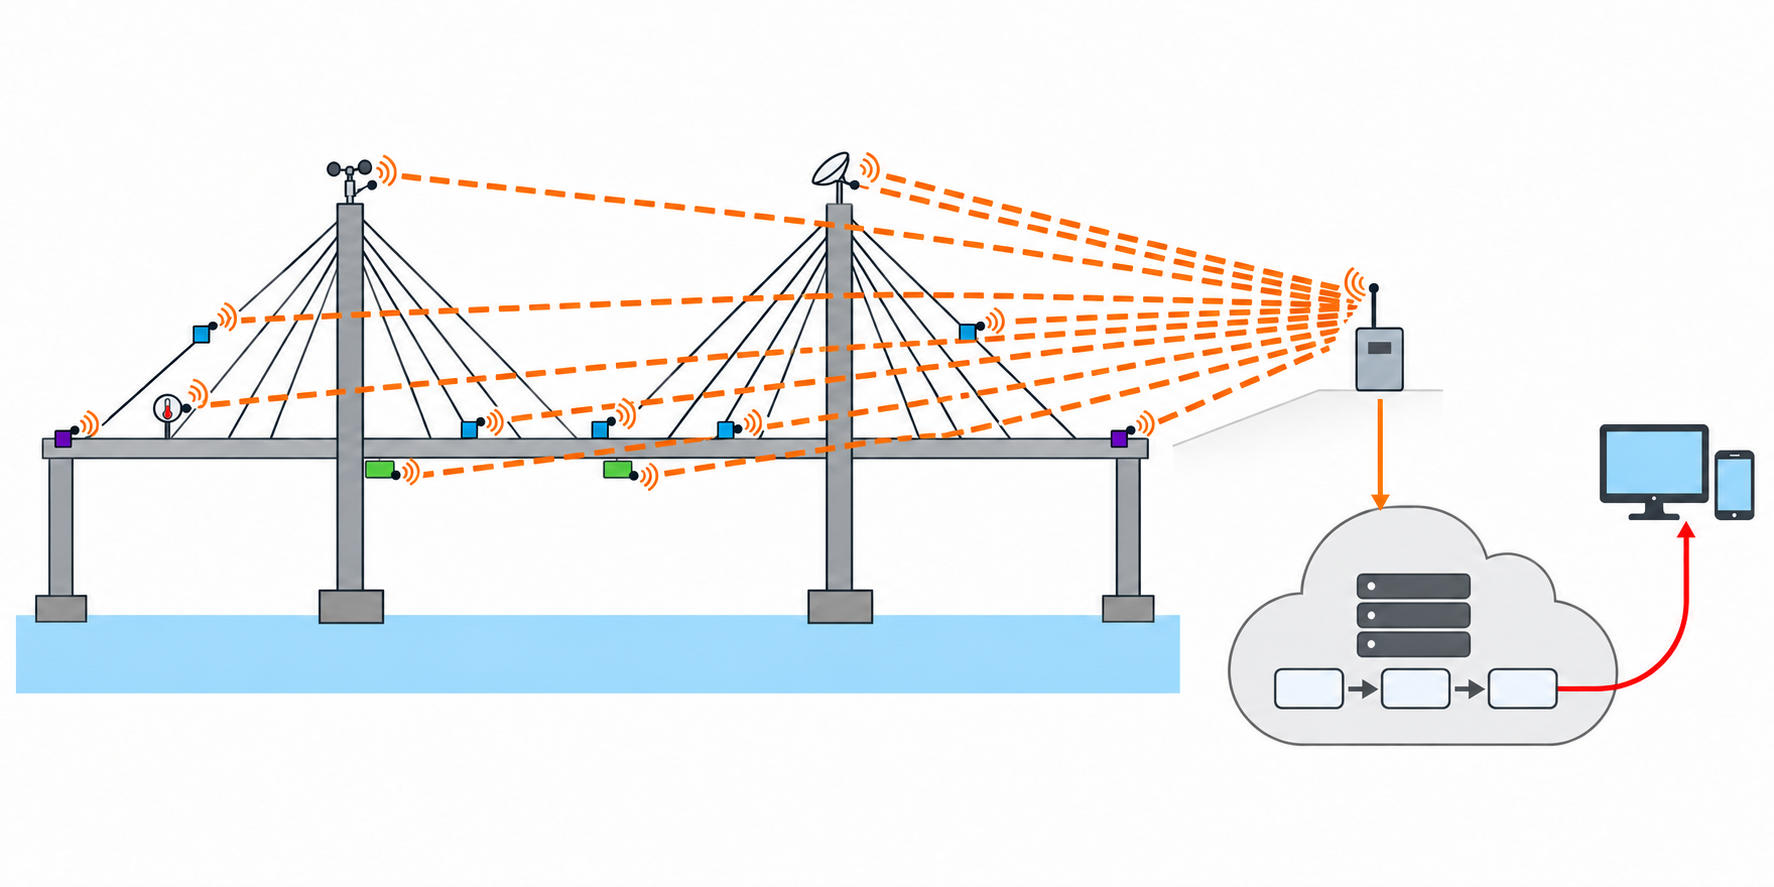
\includegraphics[width=\linewidth]{figures/ch11/ch11-06-v4-recovered.png}};
\begin{scope}[x={(img.south east)},y={(img.north west)}]
  \tikzset{
    lbl/.style={font=\sffamily\scriptsize,text=BookInk,fill=white,fill opacity=0.88,text opacity=1,inner sep=1.2pt,rounded corners=1pt,align=center},
    boxlbl/.style={font=\sffamily\tiny,text=BookInk,align=center,inner sep=0.5pt},
    ldr/.style={draw=BookInk!65,line width=0.45pt}
  }
  \node[lbl] (t1) at (0.11,0.77) {Pylon};
  \draw[ldr] (t1.east) -- (0.19,0.73);
  \node[lbl] (t2) at (0.33,0.76) {Stay cables (16 total)};
  \draw[ldr] (t2.south) -- (0.29,0.66);
  \node[lbl] (t3) at (0.56,0.42) {Deck girder};
  \draw[ldr] (t3.north) -- (0.56,0.49);
  \node[lbl,text=Ch11Orange!90!black] at (0.62,0.80) {Wireless links};
  \node[lbl] (t5) at (0.86,0.64) {On-site gateway};
  \draw[ldr] (t5.west) -- (0.80,0.61);
  \node[lbl] at (0.80,0.45) {Cloud analytics subsystem};
  \node[boxlbl] at (0.738,0.224) {Data\\[-1pt]cleaning};
  \node[boxlbl] at (0.798,0.224) {Feature\\[-1pt]extraction};
  \node[boxlbl] at (0.859,0.224) {Threshold/\\[-1pt]anomaly};
  \node[lbl,text=Ch11Red,anchor=east] (t7) at (0.985,0.58) {Alert to operators\\[-1pt]{\tiny(engineer review)}};
  \draw[draw=Ch11Red,line width=0.45pt] (t7.south) -- (0.94,0.51);

  \draw[draw=BookRule,fill=BookPale!55,rounded corners=2pt,line width=0.4pt] (0.015,0.015) rectangle (0.985,0.115);
  \node[font=\sffamily\bfseries\tiny,text=BookInk,anchor=west] at (0.022,0.082) {Sensors:};
  \filldraw[fill=Ch11Blue,draw=Ch11Gray,line width=0.4pt] (0.105,0.072) rectangle (0.117,0.092);
  \fill[black] (0.121,0.082) circle (0.0025);
  \node[font=\sffamily\tiny,text=BookInk,anchor=west] at (0.126,0.082) {Accelerometer (3 deck / 2 cable)};
  \filldraw[fill=Ch11Green,draw=Ch11Gray,line width=0.4pt] (0.380,0.074) rectangle (0.398,0.090);
  \node[font=\sffamily\tiny,text=BookInk,anchor=west] at (0.403,0.082) {Strain gauge (2)};
  \draw[Ch11Gray,line width=0.5pt] (0.535,0.070) -- (0.535,0.092);
  \draw[Ch11Gray,line width=0.5pt] (0.527,0.088) -- (0.543,0.088);
  \fill[Ch11Gray] (0.527,0.088) circle (0.003);
  \fill[Ch11Gray] (0.543,0.088) circle (0.003);
  \node[font=\sffamily\tiny,text=BookInk,anchor=west] at (0.548,0.082) {Anemometer (1)};
  \draw[Ch11Gray,fill=white,line width=0.5pt] (0.685,0.084) ellipse (0.008 and 0.005);
  \draw[Ch11Gray,line width=0.5pt] (0.685,0.071) -- (0.685,0.080);
  \node[font=\sffamily\tiny,text=BookInk,anchor=west] at (0.697,0.082) {GNSS antenna (1)};
  \draw[Ch11Gray,fill=white,line width=0.5pt] (0.855,0.082) circle (0.006);
  \node[font=\sffamily\tiny,text=BookInk,anchor=west] at (0.864,0.082) {Temp.\ (1)};

  \filldraw[fill=Ch11Purple,draw=Ch11Gray,line width=0.4pt] (0.025,0.030) rectangle (0.037,0.050);
  \node[font=\sffamily\tiny,text=BookInk,anchor=west] at (0.042,0.040) {Displacement (2)};
  \node[font=\sffamily\bfseries\tiny,text=BookInk,anchor=west] at (0.185,0.040) {Links:};
  \draw[Ch11Gray,line width=0.6pt] (0.240,0.040) -- (0.268,0.040);
  \node[font=\sffamily\tiny,text=BookInk,anchor=west] at (0.273,0.040) {Stay cable};
  \draw[Ch11Orange,dashed,line width=1.1pt] (0.375,0.040) -- (0.408,0.040);
  \node[font=\sffamily\tiny,text=BookInk,anchor=west] at (0.413,0.040) {Wireless (sensor$\rightarrow$gateway)};
  \draw[Ch11Orange,line width=1.1pt,-{Stealth[length=1.4mm]}] (0.640,0.040) -- (0.668,0.040);
  \node[font=\sffamily\tiny,text=BookInk,anchor=west] at (0.673,0.040) {WAN upload};
  \draw[Ch11Gray,line width=0.8pt,-{Stealth[length=1.3mm]}] (0.775,0.040) -- (0.798,0.040);
  \node[font=\sffamily\tiny,text=BookInk,anchor=west] at (0.803,0.040) {Analysis};
  \draw[Ch11Red,line width=1.1pt,-{Stealth[length=1.4mm]}] (0.875,0.040) -- (0.903,0.040);
  \node[font=\sffamily\tiny,text=Ch11Red,anchor=west] at (0.908,0.040) {Alert};
\end{scope}
\end{tikzpicture}
\caption{Structural health monitoring system for a cable-stayed bridge (V4 base image overlaid with TikZ labels and legend; simplified teaching architecture). Sensors on the deck, cables, and pylon tops send data through wireless nodes to an on-site gateway; the cloud cleans the data, extracts features, and checks thresholds or anomalies; alerts go to operators for engineering review. The figure does not represent a real bridge; actual systems often combine wired and wireless links, and sensor layouts depend on the design. Base art generated by an image model; labels and legend typeset with TikZ. Remaining base-image deviations are documented in Table~\ref{tab:ch11-05}.}\label{fig:ch11-06}
\end{figure}

Finally, complete the ten-item full-figure verification audit (`F1`--`F10`) in Table~\ref{tab:ch11-05}. Recording the unresolved base-image deviations transparently (narrow white cable gaps, red fill inside the thermometer, cloud below gateway, slightly undersized blue squares, and pending peer sign-off) defines the exact finishing steps required in a vector editor before journal submission.

\begin{table}[htbp]\centering\scriptsize
\setlength{\tabcolsep}{3pt}
\renewcommand{\arraystretch}{1.08}
\caption{Ten-item full-figure verification record for Figure~\ref{fig:ch11-06}.}\label{tab:ch11-05}
\begin{tabularx}{\linewidth}{@{}c>{\raggedright\arraybackslash}p{25mm}>{\raggedright\arraybackslash}p{16mm}Y>{\raggedright\arraybackslash}p{22mm}@{}}
\toprule
\textbf{\#} & \textbf{Verification item} & \textbf{Method} & \textbf{Observed result \& remaining deviations} & \textbf{Status} \\
\midrule
F1 & Twin-pylon cable-stayed bridge; no main cable & Visual check & Twin-pylon side elevation is accurate, with no suspension main cable or hangers & Passed \\
F2 & 16 stay cables connecting pylon to deck & $200\%$ count & $4+4+4+4=16$ trajectories connect pylons to deck; narrow white gaps remain behind icons/waves & Trajectories passed; bridge gaps \\
F3 & 12 sensors correct in type and location & Table audit & $3+2+2+1+1+1+2=12$ sensors in correct positions; thermometer retains red interior fill & Counts passed; remove red in thermometer \\
F4 & L1--L4 directions \& line styles correct & Trace links & All 4 link classes point in the right semantic direction; cloud sits below gateway (upload arrow points down) & Directions passed; vertical layout noted \\
F5 & Wireless links \& stay cables distinct in grayscale & Grayscale check & Thick short-dashed wireless links and thin solid stay cables remain distinct in grayscale & Passed \\
F6 & Base art text-free; labels checked word by word & $200\%$ zoom & Base bitmap contains zero text; TikZ labels and legend verified character by character & Passed \\
F7 & Icons $\ge 2\ \text{mm}$ and text $\ge 6\ \text{pt}$ at $160\ \text{mm}$ width & Scale check & TikZ text is $\ge 6\ \text{pt}$; base blue sensor squares measure $\sim 1.44\text{--}1.80\ \text{mm}$ at $160\ \text{mm}$ width & Text passed; enlarge sensor icons \\
F8 & No new collateral changes relative to V2 & Revision log & V4 preserves all pylons, stay cables, sensors, subsystems, and arrows from V2 & Passed \\
F9 & Caption states simplification \& engineer review & Read caption & Caption states ``simplified teaching architecture'' and ``alerts go to operators for engineering review'' & Passed \\
F10 & Structural engineering peer sign-off & Peer audit & Author audit complete; formal submission requires sign-off by a structural engineering colleague & Pending peer sign-off \\
\bottomrule
\end{tabularx}
\end{table}

\section{What AI Can and Cannot Do at This Stage}

Table~\ref{tab:ch11-06} summarizes the division of labor between AI tools and the author during revision and re-verification.

\begin{table}[htbp]\centering\scriptsize
\setlength{\tabcolsep}{3pt}
\renewcommand{\arraystretch}{1.08}
\caption{What AI can do, what AI cannot do, and what the author must verify during figure revision and re-verification.}\label{tab:ch11-06}
\begin{tabularx}{\linewidth}{@{}>{\raggedright\arraybackslash}p{19mm}YYY@{}}
\toprule
\textbf{Stage} & \textbf{What AI (\scidraw{}, etc.) can do} & \textbf{What AI cannot do} & \textbf{What the author must verify} \\
\midrule
Interpreting feedback & Rewrite casual remarks into itemized notes; suggest a three-level classification & Judge which items are scientific errors (requires domain knowledge and study materials) & Whether each item maps to a concrete location and object, and whether its level is correct \\
Drafting revision prompts & Turn a revision-sheet item into a clear prompt & Guarantee that the model executes only that single change & That the prompt includes both ``what to change'' and an explicit ``what must stay unchanged'' list \\
Executing edits (images) & Select a historical image in \scidraw{} (\sdtool{ai-drawing}) as a reference and iterate via prompts & Lock objects or freeze pixel regions; guarantee other objects stay unchanged & Full-figure re-verification after each edit: object counts, relations, text, and style \\
Executing edits (data plots) & Multi-turn conversational edits and one-click restore to previous/original version in \scidraw{} (\sdtool{sci-vis}) & Judge whether modified axes or encodings still represent the statistics faithfully & That data points, axes, units, and error bars still match the underlying dataset \\
Comparing versions & (External scripts) compute difference maps and side-by-side layouts & Built-in side-by-side comparison and naming (not currently in the web app; download to compare) & Manual row-by-row object counts against the inventory table; diff maps only assist \\
Rolling back & Re-select any historical image to branch again; restore prior data plots with one click & Automatically judge which version is the valid baseline & Record the baseline version and log which parent version each branch builds upon \\
Typography \& exact styles & --- & Reliable spelling, exact hex matching, or line alignment inside a bitmap & Complete labels, legends, exact colors, and line repairs in the layout layer (TikZ/vector software) \\
Logging revisions & --- & Automatically generate a traceable scientific revision log & For each version: parent, prompt text, target change, collateral changes, audit conclusion, and decision \\
\bottomrule
\end{tabularx}
\end{table}

\section{Chapter Checklist}

\begin{itemize}
\item Translate every vague comment into a ``location + observed phenomenon'' statement and assign it to Level 1 (scientific error), Level 2 (reading obstacle), or Level 3 (visual consistency).
\item Resolve Level 1 scientific errors first; when three or more scientific errors appear, rewrite the figure brief and regenerate rather than patching the broken image.
\item Restrict each row of your revision sheet to a single modification class, paired with an explicit ``must remain unchanged'' object list and verification method.
\item Delegate text labels, exact color codes, line-weight unification, and gap repairs to a deterministic layout layer (LaTeX/TikZ or vector software).
\item Re-verify the \textbf{entire figure} against your object and relation tables after every generative edit---never inspect only the edited spot.
\item Compare each new version side by side with its parent baseline, count every object row by row, and use pixel difference maps when helpful to localize changes.
\item When collateral changes occur, return to the last verified baseline and open a new branch rather than stacking patches onto the faulty version.
\item If two consecutive attempts with an explicit preservation checklist still produce collateral changes, switch routes and perform that edit in the layout layer.
\item Record the parent version, prompt text, target edit, unintended changes, and adoption decision for every version in a revision log, retaining rejected drafts.
\item Have a domain peer review and sign off on the final overlaid figure before submission.
\end{itemize}

\section{Exercises}

\begin{enumerate}
\item \textbf{Translating vague feedback (pen and paper).} Take a vague comment you recently received on a figure (or use ``This figure doesn't look professional enough''). Using the three follow-up questions from Section 11.2, write down at least six ``location + observed phenomenon'' issues, label their levels, rank them in execution order, and state which two items you would combine into one edit and which item belongs in the layout layer.
\item \textbf{Hands-on with \scidraw{}: collateral-change experiment.} In \scidraw{} (\sdtool{ai-drawing}), generate or upload a schematic from your own field as your V2 baseline, select it as a reference image, and ask to change only one line style or color. Place the resulting V3 beside V2, count all objects against your inventory table, and record whether the target edit succeeded and whether any collateral changes occurred. Then return to V2, attach an explicit preservation checklist to the same edit, compare both outcomes, and compile a revision log formatted like Table~\ref{tab:ch11-04}.
\item \textbf{Data-plot revision comparison.} Upload a public or synthetic dataset into \scidraw{} Scientific Visualization (\sdtool{sci-vis}), generate a chart, apply three sequential edits (e.g., palette, axis range, legend position), and restore the previous and original versions. Write a 200-word note explaining how editing and rollback in data plots differ from generative edits in schematics, and why both still require full-figure re-verification.
\end{enumerate}

\section*{References}

{\sloppy
\begin{itemize}
\item Farrar CR, Worden K. An introduction to structural health monitoring. \textit{Philosophical Transactions of the Royal Society A}. 2007;365(1851):303--315. doi:10.1098/rsta.2006.1928
\item Kim S, Pakzad S, Culler D, Demmel J, Fenves G, Glaser S, Turon M. Health monitoring of civil infrastructures using wireless sensor networks. In: \textit{Proceedings of the 6th International Conference on Information Processing in Sensor Networks (IPSN '07)}. ACM; 2007:254--263. doi:10.1145/1236360.1236395
\item Ko JM, Ni YQ. Technology developments in structural health monitoring of large-scale bridges. \textit{Engineering Structures}. 2005;27(12):1715--1725. doi:10.1016/j.engstruct.2005.02.021
\item Lynch JP, Loh KJ. A summary review of wireless sensors and sensor networks for structural health monitoring. \textit{The Shock and Vibration Digest}. 2006;38(2):91--128. doi:10.1177/0583102406061499
\item Rougier NP, Droettboom M, Bourne PE. Ten simple rules for better figures. \textit{PLoS Computational Biology}. 2014;10(9):e1003833. doi:10.1371/journal.pcbi.1003833
\item Wong B. Simplify to clarify. \textit{Nature Methods}. 2011a;8(8):611. doi:10.1038/nmeth.1660
\item Wong B. Points of view: Color blindness. \textit{Nature Methods}. 2011b;8(6):441. doi:10.1038/nmeth.1618
\end{itemize}
\par}

% TODO: figures/ch11/ch11-03-v2-brief.png and figures/ch11/ch11-06-v4-recovered.png retain 4 known base-image deviations (cloud positioned below gateway, red interior fill in the thermometer icon, blue sensor squares measuring ~1.44-1.80 mm at 160 mm width, and narrow white halo gaps where stay cables pass behind icons); these are documented transparently in the text and in Tables 11-3, 11-4, and 11-5.
% TODO: figures/ch11/ch11-05-diff-and-count-en.pdf currently contains the Chapter 7 difference heatmap row and the two-case object count table (with the bottom border of the final table row slightly clipped); if the script is re-run later to add the Chapter 11 V2/V3 difference heatmap row, update the Figure 11-5 caption accordingly.
% TODO: figures/ch11/ch11-08-version-tree-en.tex labels node V3 as "Collateral change (rejected)"; the body text and Figure 11-8 caption explain that this branch illustrates the standard rollback logic when collateral changes occur.
